%%% The main file. It contains definitions of basic parameters and includes all other parts.

%% Settings for single-side (simplex) printing
% Margins: left 40mm, right 25mm, top and bottom 25mm
% (but beware, LaTeX adds 1in implicitly)
\documentclass[12pt,a4paper,dvipsnames]{report}
\setlength\textwidth{145mm}
\setlength\textheight{247mm}
\setlength\oddsidemargin{15mm}
\setlength\evensidemargin{15mm}
\setlength\topmargin{0mm}
\setlength\headsep{0mm}
\setlength\headheight{0mm}
% \openright makes the following text appear on a right-hand page
\let\openright=\clearpage

%% Settings for two-sided (duplex) printing
% \documentclass[12pt,a4paper,twoside,openright]{report}
% \setlength\textwidth{145mm}
% \setlength\textheight{247mm}
% \setlength\oddsidemargin{14.2mm}
% \setlength\evensidemargin{0mm}
% \setlength\topmargin{0mm}
% \setlength\headsep{0mm}
% \setlength\headheight{0mm}
% \let\openright=\cleardoublepage

%% Generate PDF/A-2u
\usepackage[a-2u]{pdfx}

%% Character encoding: usually latin2, cp1250 or utf8:
\usepackage[utf8]{inputenc}

%% Prefer Latin Modern fonts
\usepackage{lmodern}

%% CUSTOMIZATION: Support diacritics
\usepackage[T1]{fontenc}
\usepackage{textcomp}

%% Further useful packages (included in most LaTeX distributions)
\usepackage{amsmath}        % extensions for typesetting of math
\usepackage{amsfonts}       % math fonts
\usepackage{amsthm}         % theorems, definitions, etc.
\usepackage{bbding}         % various symbols (squares, asterisks, scissors, ...)
\usepackage{bm}             % boldface symbols (\bm)
\usepackage{graphicx}       % embedding of pictures
\usepackage{fancyvrb}       % improved verbatim environment
\usepackage[sort&compress]{natbib}         % citation style AUTHOR (YEAR), or AUTHOR [NUMBER]
\usepackage[nottoc]{tocbibind} % makes sure that bibliography and the lists
			    % of figures/tables are included in the table
			    % of contents
\usepackage{dcolumn}        % improved alignment of table columns
\usepackage{booktabs}       % improved horizontal lines in tables
\usepackage{paralist}       % improved enumerate and itemize
\usepackage{xcolor}         % typesetting in color

\ifdefined\version\ifx\version\empty\else
	\usepackage{background}
	\SetBgContents{\version}
	\SetBgScale{1}
	\SetBgAngle{0}
	\SetBgOpacity{1}
	\SetBgColor{gray}
	\SetBgPosition{current page.south west}
	\SetBgAnchor{right}
	\SetBgHshift{.5cm}
	\SetBgVshift{.5cm}
\fi\fi

\usepackage{bold-extra}
\usepackage{wrapfig}
\usepackage{qrcode}
\usepackage{xurl}
\usepackage{float}
\usepackage{import}
\usepackage{listings}
\lstset{
  basicstyle=\ttfamily,
  columns=fixed,
  fontadjust=true,
  basewidth=0.5em,
  showstringspaces=false,
}
\definecolor{gray}{rgb}{0.4,0.4,0.4}
\definecolor{darkblue}{rgb}{0.0,0.0,0.6}
\definecolor{cyan}{rgb}{0.0,0.6,0.6}
\lstdefinelanguage{XML}
{
  morestring=[b]",
  morestring=[s]{>}{<},
  morecomment=[s]{<?}{?>},
  stringstyle=\color{black},
  identifierstyle=\color{darkblue},
  keywordstyle=\color{cyan},
  morekeywords={xmlns,version,type}% list your attributes here
}
\lstdefinelanguage{json}{
    literate=
     *{0}{{{\color{numb}0}}}{1}
      {1}{{{\color{numb}1}}}{1}
      {2}{{{\color{numb}2}}}{1}
      {3}{{{\color{numb}3}}}{1}
      {4}{{{\color{numb}4}}}{1}
      {5}{{{\color{numb}5}}}{1}
      {6}{{{\color{numb}6}}}{1}
      {7}{{{\color{numb}7}}}{1}
      {8}{{{\color{numb}8}}}{1}
      {9}{{{\color{numb}9}}}{1}
      {:}{{{\color{punct}{:}}}}{1}
      {,}{{{\color{punct}{,}}}}{1}
      {\{}{{{\color{delim}{\{}}}}{1}
      {\}}{{{\color{delim}{\}}}}}{1}
      {[}{{{\color{delim}{[}}}}{1}
      {]}{{{\color{delim}{]}}}}{1},
}
\usepackage{tikz}
\usepackage[multiple]{footmisc}
\usepackage{tikzpeople}
\usetikzlibrary{positioning}
\usetikzlibrary{shadows}
\usetikzlibrary{shapes.geometric,shapes.misc,decorations.pathreplacing,calligraphy}
\tikzset{%
  squarednode/.style={rectangle, draw=CadetBlue!60, fill=CadetBlue!5, very thick, minimum size=5mm,align=center},
  %
  module/.style={rectangle, draw=CadetBlue!60, fill=CadetBlue!5, very thick, minimum size=5mm,align=center},% as application
  dataSpecification/.style={rectangle, draw=Fuchsia!60, fill=Fuchsia!5, very thick, minimum size=5mm,align=center},% our new concept
  schema/.style={rectangle, draw=MidnightBlue!60, fill=MidnightBlue!5, very thick, minimum size=5mm,align=center},% artifact, but is schema
  artefact/.style={rectangle, draw=Periwinkle!60, fill=Periwinkle!5, very thick, minimum size=5mm,align=center},% general artifact
  document/.style={rectangle, draw=Periwinkle!60, fill=Periwinkle!5, very thick, minimum size=5mm,align=center},% general artifact
  mapping/.style={rectangle, draw=Black!60, fill=Black!5, very thick, minimum size=5mm,align=center},
  seda/.style={rectangle, draw=Gray!60, fill=Gray!5, very thick, minimum size=5mm,align=center},
  % ---
  % CIM
  % ---
  ontology/.style={rectangle, draw=RedViolet!60, fill=RedViolet!5, very thick, minimum size=5mm,align=center},% ontology or CIM
  %
  ontologyClass/.style={shape=rectangle, draw=violet!60, fill=violet!5, very thick, minimum size=5mm,align=center},
  % ----------------------------------
  % PIM entities used only to show PIM
  % ----------------------------------
  pimClass/.style={rectangle, draw=violet!60, fill=violet!5, very thick, minimum size=5mm,align=center},
  pimAttribute/.style={rectangle, draw=teal!60, fill=teal!5, very thick, minimum size=5mm,align=center},
  pimAssociation/.style={rectangle, draw=purple!60, fill=purple!5, very thick, minimum size=5mm,align=center},
  pimAssociationend/.style={rectangle, draw=pink!60, fill=pink!5, very thick, minimum size=5mm,align=center},
  % -----------------------------
  % PSM entities to show only PSM
  % -----------------------------
  generalSchema/.style={rectangle, draw=blue!60, fill=blue!5, very thick, minimum size=5mm,align=center},% equivalent to PSM
  %
  psmClass/.style={rectangle, draw=Orchid!60, fill=Orchid!5, very thick,align=center},
  psmAttribute/.style={rectangle, draw=OliveGreen!60, fill=OliveGreen!5, very thick,align=center},
  psmOr/.style={diamond, draw=Thistle!60, fill=Thistle!5, very thick,align=center},
  psmOrGroup/.style={circle, draw=Thistle!60, fill=Thistle!5, very thick, minimum size=5mm,align=center},
  psmIncludes/.style={chamfered rectangle, draw=Magenta!60, fill=Magenta!5, very thick,align=center},
  %
  human/.style={,minimum size=.8cm},
  database/.style={
      cylinder,
      cylinder uses custom fill,
      cylinder body fill=yellow!50,
      cylinder end fill=yellow!50,
      shape border rotate=90,
      aspect=0.25,
      draw
   },
  %
  cascaded/.style = {%
    general shadow = {%
      shadow scale = 1,
      shadow xshift = 1ex,
      shadow yshift = -1ex,
      draw,
      fill = white},
    general shadow = {%
      shadow scale = 1,
      shadow xshift = .5ex,
      shadow yshift = -.5ex,
      draw,
      fill = white}}}
\usepackage{ amssymb }
\usepackage[inline]{enumitem}

\theoremstyle{definition}
\newtheorem{requirement}{Requirement}
\newcommand{\requirementautorefname}{Requirement}
\newtheorem{definition}{Definition}
\newtheorem*{notation}{Notation}
\usepackage{tabularx}
\usepackage{makecell}

\usepackage{caption}
\usepackage{subcaption}
\usepackage{xcolor}
\newcommand{\td}[1]{\bigskip\par\noindent{\color{purple}#1}\par\bigskip}

%\usepackage[textcolor=purple,color=purple,bordercolor=white,backgroundcolor=white,size=tiny]{todonotes}\marginpar{left}
%\reversemarginpar
%\geometry{marginparwidth=75pt}
\usepackage[super]{nth}

\usepackage{afterpage}
\usepackage{pdflscape}
\usepackage{dsfont}
\usepackage{xhfill}
\usepackage[skins]{tcolorbox}
\usepackage{varwidth}
\makeatletter
\newtcolorbox{mybox}[1][]{
  enhanced,
  colframe=black, colback=white,
  sharp corners,
  boxrule=0.6pt,
  detach title,
  coltitle=black,
  colbacktitle=white,
  fonttitle=\footnotesize,
  enlarge left by=-8mm,
  enlarge right by=-2mm,
  width=\linewidth+10mm,
  left=7mm,
  right=2mm,
  before upper=\setlength{\parindent}{17.62482pt}\everypar{{\setbox0\lastbox}\@minipagefalse\everypar{}},
%  overlay={
%    \node[rotate=90,
%          fill=tcbcolbacktitle,
%          font=\kvtcb@fonttitle,
%          minimum width=1cm]
%          at (frame.west)
%      {\begin{varwidth}{\tcbtextheight}%
%         \centering\tcbtitle\par
%       \end{varwidth}};
%  },
#1}
\makeatother

% \newenvironment{showcase}
% {\bigskip\begin{mybox}[title=Example]}
% {\end{mybox}\bigskip}

\newenvironment{showcase}
{\bigskip}
{\bigskip}


%%% Basic information on the thesis

% Thesis title in English (exactly as in the formal assignment)
\def\ThesisTitle{Model-driven approach for data schema definitions modeling}

% Author of the thesis
\def\ThesisAuthor{Bc. Štěpán Stenchlák}

% Year when the thesis is submitted
\def\YearSubmitted{2022}

% Name of the department or institute, where the work was officially assigned
% (according to the Organizational Structure of MFF UK in English,
% or a full name of a department outside MFF)
\def\Department{Department of Software Engineering}

% Is it a department (katedra), or an institute (ústav)?
\def\DeptType{Department}

% Thesis supervisor: name, surname and titles
\def\Supervisor{doc. Mgr. Martin Nečaský, Ph.D.}

% Supervisor's department (again according to Organizational structure of MFF)
\def\SupervisorsDepartment{Department of Software Engineering}

% Study programme and specialization
\def\StudyProgramme{Computer Science - Software and Data Engineering (N0613A140015)}
\def\StudyBranch{Computer Science - Software and Data Engineering}

% An optional dedication: you can thank whomever you wish (your supervisor,
% consultant, a person who lent the software, etc.)
\def\Dedication{%
This thesis was made possible thanks to numerous people who helped me or motivated me during the journey.

On the one side, I would like to thank my family for the financial support and for encouraging me to continue educating myself. Thanks to my girlfriend Kateřina for all the emotional support despite the long nights spent on this project.

I want to express my gratitude to my supervisor, doc. Mgr. Martin Nečaský, Ph.D., for guiding me through this and other projects during my study and helping me find the right branch of informatics I enjoy exploring. I also value the help from my consultants Mgr. Petr Škoda, Ph.D. and RNDr. Jakub Klímek, Ph.D.

Finally, I want to thank my friend Jáchym Bártík for the long-lasting friendly rivalry, which will continue in our Ph.D. study.
}

% Abstract (recommended length around 80-200 words; this is not a copy of your thesis assignment!)
\def\Abstract{%
This work analyzes, formalizes, and implements a framework for multi-level conceptual modeling of various serialization formats based on Model-Driven Architecture and previously developed tools XCase and eXolutio. It enables users to model their schema from a conceptual model in one general form from which multiple schema formats can be derived alongside documentation and transformation scripts. The thesis introduces base formalisms and findings and analyzes advanced requirements for the following work in this area, such as evolution and inheritance of schemas.

The primary use case of the tool is modeling formal open standards for publishing open data for the Czech government and public institutions. Nevertheless, the intent is to make the tool for general schema modeling.
}

% 3 to 5 keywords (recommended), each enclosed in curly braces
\def\Keywords{%
{schema definition} {data modeling} {ontologies} {Model-Driven Architecture}
}

%% The hyperref package for clickable links in PDF and also for storing
%% metadata to PDF (including the table of contents).
%% Most settings are pre-set by the pdfx package.
\hypersetup{unicode}
\hypersetup{breaklinks=true}

% Definitions of macros (see description inside)
%%% This file contains definitions of various useful macros and environments %%%
%%% Please add more macros here instead of cluttering other files with them. %%%

%%% Minor tweaks of style

% These macros employ a little dirty trick to convince LaTeX to typeset
% chapter headings sanely, without lots of empty space above them.
% Feel free to ignore.
\makeatletter
\def\@makechapterhead#1{
  {\parindent \z@ \raggedright \normalfont
   \Huge\bfseries \thechapter. #1
   \par\nobreak
   \vskip 20\p@
}}
\def\@makeschapterhead#1{
  {\parindent \z@ \raggedright \normalfont
   \Huge\bfseries #1
   \par\nobreak
   \vskip 20\p@
}}
\makeatother

% This macro defines a chapter, which is not numbered, but is included
% in the table of contents.
\def\chapwithtoc#1{
\chapter*{#1}
\addcontentsline{toc}{chapter}{#1}
}

% Draw black "slugs" whenever a line overflows, so that we can spot it easily.
\overfullrule=1mm

%%% Macros for definitions, theorems, claims, examples, ... (requires amsthm package)

\theoremstyle{plain}
\newtheorem{thm}{Theorem}
\newtheorem{lemma}[thm]{Lemma}
\newtheorem{claim}[thm]{Claim}

\theoremstyle{plain}
\newtheorem{defn}{Definition}

\theoremstyle{remark}
\newtheorem*{cor}{Corollary}
\newtheorem*{rem}{Remark}
\newtheorem*{example}{Example}

%%% An environment for proofs

\newenvironment{myproof}{
  \par\medskip\noindent
  \textit{Proof}.
}{
\newline
\rightline{$\qedsymbol$}
}

%%% An environment for typesetting of program code and input/output
%%% of programs. (Requires the fancyvrb package -- fancy verbatim.)

\DefineVerbatimEnvironment{code}{Verbatim}{fontsize=\small, frame=single}

%%% The field of all real and natural numbers
\newcommand{\R}{\mathbb{R}}
\newcommand{\N}{\mathbb{N}}

%%% Useful operators for statistics and probability
\DeclareMathOperator{\pr}{\textsf{P}}
\DeclareMathOperator{\E}{\textsf{E}\,}
\DeclareMathOperator{\var}{\textrm{var}}
\DeclareMathOperator{\sd}{\textrm{sd}}

%%% Transposition of a vector/matrix
\newcommand{\T}[1]{#1^\top}

%%% Various math goodies
\newcommand{\goto}{\rightarrow}
\newcommand{\gotop}{\stackrel{P}{\longrightarrow}}
\newcommand{\maon}[1]{o(n^{#1})}
\newcommand{\abs}[1]{\left|{#1}\right|}
\newcommand{\dint}{\int_0^\tau\!\!\int_0^\tau}
\newcommand{\isqr}[1]{\frac{1}{\sqrt{#1}}}

%%% Various table goodies
\newcommand{\pulrad}[1]{\raisebox{1.5ex}[0pt]{#1}}
\newcommand{\mc}[1]{\multicolumn{1}{c}{#1}}


% Title page and various mandatory informational pages
\begin{document}
%%% Title page of the thesis and other mandatory pages

%%% Title page of the thesis

\pagestyle{empty}
\hypersetup{pageanchor=false}
\begin{center}

\centerline{\mbox{
\includegraphics[width=166mm]{img/logo-en.pdf}}}

\vspace{-8mm}
\vfill

{\bf\Large MASTER THESIS}

\vfill

{\LARGE\ThesisAuthor}

\vspace{15mm}

{\LARGE\bfseries\ThesisTitle}

\vfill

\Department

\vfill

{
\centerline{\vbox{\halign{\hbox to 0.45\hsize{\hfil #}&\hskip 0.5em\parbox[t]{0.45\hsize}{\raggedright #}\cr
Supervisor of the master thesis:&\Supervisor \cr
\noalign{\vspace{2mm}}
Study programme:&\StudyProgramme \cr
\noalign{\vspace{2mm}}
Study branch:&\StudyBranch \cr
}}}}

\vfill

% Zde doplňte rok
Prague \YearSubmitted

\end{center}

\newpage

%%% Here should be a bound sheet included -- a signed copy of the "master
%%% thesis assignment". This assignment is NOT a part of the electronic
%%% version of the thesis. DO NOT SCAN.

%%% A page with a solemn declaration to the master thesis

\openright
\hypersetup{pageanchor=true}
\pagestyle{plain}
\pagenumbering{roman}
\vglue 0pt plus 1fill

\noindent
I declare that I carried out this master thesis independently, and only with the cited
sources, literature and other professional sources. It has not been used to obtain another
or the same degree.

\medskip\noindent
I understand that my work relates to the rights and obligations under the Act No.~121/2000 Sb.,
the Copyright Act, as amended, in particular the fact that the Charles
University has the right to conclude a license agreement on the use of this
work as a school work pursuant to Section 60 subsection 1 of the Copyright~Act.

\vspace{10mm}

\hbox{\hbox to 0.5\hsize{%
In \hbox to 6em{\dotfill} date \hbox to 6em{\dotfill}
\hss}\hbox to 0.5\hsize{\dotfill\quad}}
\smallskip
\hbox{\hbox to 0.5\hsize{}\hbox to 0.5\hsize{\hfil Author's signature\hfil}}

\vspace{20mm}
\newpage

%%% Dedication

\openright

\noindent
\Dedication

\newpage

%%% Mandatory information page of the thesis

\openright

\vbox to 0.5\vsize{
\setlength\parindent{0mm}
\setlength\parskip{5mm}

Title:
\ThesisTitle

Author:
\ThesisAuthor

\DeptType:
\Department

Supervisor:
\Supervisor, \SupervisorsDepartment

Abstract:
\Abstract

Keywords:
\Keywords

\vss}

\newpage

\openright
\pagestyle{plain}
\pagenumbering{arabic}
\setcounter{page}{1}


%%% A page with automatically generated table of contents of the master thesis

\tableofcontents

%%% Each chapter is kept in a separate file
\chapter*{Introduction}
\addcontentsline{toc}{chapter}{Introduction}

%% todo: ty protocols jsou rules a napojit to na ty ofnka
% Priklad predelat jen na JSON, to XML tam nedava smysl. Vzpomen si na priklad se SISem

During the software development process, we may come to a point where splitting a large codebase into smaller, well-defined chunks is necessary to maintain the growth of our software. Using existing systems and connecting them is also a viable approach to building software. In both cases, we end up with many applications and services working together.

This approach reduces complexity and demands on software developers as each part can be maintained, deployed, and tested separately. Each developer team must know only the portion they maintain and the immediate surrounding. The surrounding is then defined by a set of rules - an agreement specifying the data which flows between the systems.

Those rules must be created, documented, and maintained, which can be a long, error-prone task. The result of the process is usually a set of data schemas and a documentation for developers. Especially the schemas need to be designed carefully to be, if possible, consistent in format and naming.

\begin{showcase}

As an example, consider a company selling and distributing its own goods. The goods are stored in warehouses and then shipped to customers. For the shipping process, the warehouse workers need to know the properties of the items they need to send. Similarly, customers need to know the properties of items they are buying. This scenario is denoted in the following image. The nodes are individual systems in the company that communicate with each other.

\bigskip

\begin{center}
    \begin{tikzpicture}[
        squarednode/.style={rectangle, draw=purple!60, fill=purple!5, very thick, minimum size=5mm},
    ]
        %Nodes
        \node[squarednode] (db) {Company's goods database};
        \node[squarednode] (warehouse) [below=2cm of db, xshift=.5cm,anchor=north west] {Warehouse application};
        \node[squarednode] (shop) [below=2cm of db, xshift=-.5cm,anchor=north east] {Online shop};

        %Lines
        \draw[-latex] (db) -- node[text width=3cm,align=center,auto,anchor=west,midway]{order info with items to send} (warehouse);
        \draw[-latex] (db) -- node[text width=3.5cm,align=center,auto,anchor=east,midway]{list of available items} (shop);
    \end{tikzpicture}
\end{center}

We need to made two "agreements": one for the warehouse and one for the online shop. Although both describe the item, the warehouse may require only the \textit{name} and \textit{weight} of the items, contrary to the online shop where the \textit{price} is also essential.

\end{showcase}

Our goal is to describe the schemas and all the rules formally. We want to specify which system sends which data and in which format. By doing this without any tool, we may find several obstacles during the process:

\begin{enumerate}
    \item We may need to describe the same thing for every schema that uses it. Hence doing the \textbf{same work multiple times}. \textit{In the example the item is used in two different schemas.}
    \item There is a high chance of \textbf{inconsistency}. We may name the semantically identical things differently, which may confuse software engineers who came in touch with multiple system parts. \textit{For example, the "name" of the item sold can be interchanged with "label" or "title".}
    \item We \textbf{lack context} in the whole system where the entities are used. \textit{It is hard to tell which systems operate with things and what will be impacted if something changes.}
\end{enumerate}

In addition to these obstacles, it is hard to provide supporting documentation, diagrams, and examples.

\begin{showcase} %N Tohle by mělo být ještě rozvedeno, klidně jako Example 2, kde ukážete ty artefakty, které musejí být vytvořeny. tj. nějaké kousky dvou různých schémat (stačí schematicky/vizuálně), diagramů, dokumentačních textů, příkladů - jen naznačit. Ale ukázat a vysvětlit trochu detailněji. Toto je opravdu moc stručné a hodně od čtenáře předpokládáte. To dost snižuje readability.
As an example, lets focus on the data between the database and the online shop. We use schemas to formally describe the data. In this case, the requirement may be to use JSON format.

\begin{verbatim}
{
  "$schema": "https://json-schema.org/draft/2020-12/schema",
  "title": "Item",
  "description": "Single item that can be sold in the store.",
  "type": "object",
  "required": [],
  "properties": {
    "name": {
      "type": "string",
      "title": "Item name"
    },
    "price": {
      "type": "object",
      "title": "price",
      ...
    }
  }
}
\end{verbatim}

The \textbf{documentation} then would describe each property of the schema in more detail in human-readable form. For example, the \textit{name} of the item may not contain a category of the item, therefore it would be necessary to always include a photo, or the type of the item to get the context.

\textbf{Diagrams} may be handy to show the full structure of the data similarly as the diagram in the previous example. People who will work with the data may use the diagrams to understand the problematics easily.

\textbf{Examples} of the data that may be send between the system are also valuable piece of information, as most of the domain logic is simple enough to infer it from the example. In our case, \textit{name} and \textit{price} are self-explanatory and we may be only interested in how to represent them to be valid.
\end{showcase}

Future modifications to the system or changes in user requirements may enforce altering the schemas, which again may require changing the same thing multiple times and may cause inconsistency. Formally, we will denote changing of schemas as an \textbf{evolution}. The process of evolution is complex, as there can already be existing data that conform to the changed schemas. In that scenario, properly implementing a change in a user requirement requires modifying affected schemas, documentation, and all the data (in case the data are stored in the given format).

\begin{showcase}
    As an example, suppose that the address provided by a customer to deliver the goods is represented in multiple parts as \textit{street}, \textit{city}, \textit{zip code}, etc. We may decide that it would be better to have everything in one field as some parts of the address may be missing or not granular enough. The evolution in this case would mean to change all the schemas, documentation and examples to reflect the new structure, and possibly create transformation scripts to convert old data to the new format.
\end{showcase}

\section*{Ontology}
\addcontentsline{toc}{section}{Ontology}
%N Nerozumím, co tady znamená to "tends us". Jako že nás příklad vede k nějakému formálnímu popisu? Moc tomu nerozumím. Ale řekl bych spíš, že ten příklad naznačuje, že problém návrhu interfaců v komplexním systému (tj. systému, který má více než jeden interface) je potřeba vnímat na dvou rovinách - technická rovina definice datových struktur a jejich popisu a konceptuální / ontologická rovina nad tím, která zachycuje věcnou podstatu bez technických detailů. A že tato rovina se obvykle vyjadřuje v podobě ontologie.

The full process of designing of schemas need to be percieved on two levels. (i) On a technical level, where a user creates the schemas and describes the rules, (ii) and on conceptual level, where the things and the relations between them are defined. The later level is called an \textbf{ontology}.

An ontology describes and names relations between the concepts from a real life without the technical details. Concepts are \textit{order}, \textit{customer}, or \textit{goods} in our case. Relations then specify, for example, that \textit{the order belongs to a customer} and \textit{consists of goods}.

With the data on the web \cite{data-on-the-web} trend in the last few years, even ontologies are becoming accessible publicly. Popular formats include RDFS (or RDF Schema), OWL, UFO, schema.org, and Wikidata. For example, schema.org is a proprietary format describing useful data for search engines, such as events, organizations, or places.

Using pre-defined ontologies in a semi-automatic way of defining schemas is beneficiary because a schema designer may focus entirely on the schema structure and not on the domain semantics.

\section*{Motivation}
\addcontentsline{toc}{section}{Motivation}

% Není jasné, proč tato sekce. Jak se to váže k předchozímu? Není spíš lepší OFNky použít jako motivaci? Tj. pojmenovat tu sekci jako "Motivation" a říci, že výše uvedený příklad je jednoduchý umělý příklad, který demonstruje problém. A říci, že ale máme silnější motivaci a tou je reálný problém návrhu OFN - říci co je OFN, což jste udělal. Ale pak to lépe navázat na text a pojmy výše, to tam teď chybí.

The example above is a simple demonstration of the problematics behind the data modelling. This chapter show stronger motivation for the same problem.

\smallskip

\textbf{Open data} is a term for data published on the web without any restrictions on use. This means that anyone can use, modify and distribute the data for any reason, including commercial use.

The definition of open data is very loose but can be further specified by a 5-star scheme designed by Sir Tim Berners-Lee. Each star adds a restriction up until the fifth star describing the Linked Open Data.
\begin{itemize}[noitemsep,leftmargin=2cm]
    \item [1 $\bigstar$] Data are published on the web and can be used freely.
    \item [2 $\bigstar$] Data are structured and in a machine-readable format.
    \item [3 $\bigstar$] The format is not proprietary; hence anyone can open them.
    \item [4 $\bigstar$] Data uses RDF and SPARQL standards from W3C.
    \item [5 $\bigstar$] Data are linked to other data creating a network of data.
\end{itemize}

\smallskip

According to the directive 2019/1024 of the European Parliament, data of public institutions shall be published as open data on the Internet in all formats it was created, and if possible, in a machine-readable format. This description corresponds to two stars in the schema above.

%N Blbé je, že to není v angličtině. Lepší odkázat na úplně původní zdroj toho pojmu, což je EU legislativa - https://eur-lex.europa.eu/legal-content/en/TXT/?uri=CELEX%3A32019L1024 - tam Article 2, bod 15 . V angličtině je to navíc Formal Open Standard (FOS), takže v angl. textu používat toto. Překlad do češtiny vyplývá z české verze toho EU materiálu : https://eur-lex.europa.eu/legal-content/CS/TXT/HTML/?uri=CELEX:32019L1024&from=en

The act then specifies \textbf{FOSes}\footnote{\url{https://eur-lex.europa.eu/legal-content/en/TXT/?uri=CELEX\%3A32019L1024}} \textit{(Formal Open Standard)} as recommendations for publishing selected categories of data, such as information about \textit{Tourist destinations} and \textit{Sports centers}. The purpose of these documents is to standardize how these data are published, usually by defining JSON and XML schemas along with textual documentation.

Until recently, all those recommendations (OFNs) were created by hand without any tool.

\smallskip

The process of designing those recommendations is comparable to designing schemas for a software system mentioned above - the designer needs to create schemas and documentation for them with examples and images.

\section*{Focus of the work}
\addcontentsline{toc}{section}{Focus of the work}

This thesis will analyze and extend\footnote{The author implemented the basis of the tool as his research project. This thesis, therefore, introduces advanced constructs and formalizes those already implemented.} a newly created tool, Dataspecer \cite{dataspecer}, and formally define and analyze its internal model, which follows previous research in the XML data modeling area and extends it to support new requirements.

Due to the complexity of the topic, this thesis does not attempt to cover and implement all details, as some of them will be analyzed by future work. The thesis only focuses on the current author's work and formalizes the basics.

Dataspecer is a web tool for effortless creation and management of data specifications, such as XSD, JSON Schema, and CSV Schema, and the creation of supplementary documents. The tool helps the user model schemas by providing relations from the chosen ontology. Schemas are modeled in a graphical interface in the form of the tree, which is then converted to various schemas.

Supplementary documents are automatically generated files from the modeled schemas, such as:

\begin{itemize}
    \item \textbf{documentation} - Human-readable description of entities from the ontology, that are used in the schema as well as description of the schema.
    \item \textbf{data transformations} - Scripts that can convert data from one schema to another, even between different technologies, such as JSON and XML.
    \item \textbf{examples} - Small datasets that can be used instead of the documentation to understand the schema.
    \item \textbf{example application} - Depending on the context of modeled schema, if the schema describes web-accessible data, it is possible to generate a web application that uses those data as a proof that the workflow works.
\end{itemize}

The tool is already in use for creating new schemas for the public sector of the Czech Republic, including the OFNs.

\bigskip

\noindent The rest of the thesis is organized as follows.

\begin{itemize}
    \item The following chapter \ref{chapters:related-work} analyzes related work and introduces the previous works as the common ground this work will follow - precisely the model-driven approach for data modeling and evolution of XML documents.
    \item Chapter \ref{chapters:analysis} briefly analyzes new requirements for the software as many requirements were already studied in the related work. The chapter focuses on support for schemas other than XML and the data on the web \cite{data-on-the-web} approach to ontology and the modeled schemas.
    It also defines the internal model to represent schemas and changes from the related work where it was first introduced. Changes are also analyzed concerning the new requirements.
    \item The next chapter \ref{chapters:implementation} then briefly describes how this model is integrated into the Dataspecer tool.
    \item The last chapter \ref{chapters:future-work} introduces and briefly analyzes topics for future work, such as the change propagation (evolution) in schemas.
\end{itemize}


\chapter{Previous research}
\label{chapters:previous-research}

This short chapter introduces the core concepts of the previous research that was carried out by the \textit{XML and Web Engineering Research Group} (XRG) at the Faculty of Mathematics and Physics of the Charles University in the years 2012 to 2015. Those concepts will be used for further analysis in the following chapters.

\bigskip

In 2012 XRG formalized a novel approach\footnote{The work builds on previous work of the same authors where they introduced the XSEM model \cite{necasky2007xsem}, which has later been a subject of their study.} to modeling XML schemas \cite{necasky2012conceptual} for a particular domain ontology by integrating Model Driven Development \cite{kent2002model} (specifically Model Driven Architecture) techniques to separate a conceptual mo\-del describing the domain ontology and a structural model which described the concrete XML schema.

\paragraph{Model-Driven Architecture} MDD is a software engineering technique that abstracts software development into several levels (models) to allow flexibility by separating business domain from platform decisions. MDA \cite{mda,mda_developing_in} introduced by Object Management Group (OMG) is a specialization of MDD focusing on the automation of the development of software systems.

MDA introduces four models. The topmost level CIM (Computation Independent Model) expresses the business logic and has no formal representation, as it is only a concept, hence the name computation independent. PIM (Platform Independent Model) as a second level models the business logic in UML. It does not specify a concrete platform or technology, but only the concepts in a formalized way. PSM (Platform Specific Model) reflects the formalized concepts from PIM in a platform-specific environment, such as in XML Schema, C\# or Java code, or a database schema.

The key concept is a transformation as the process of mapping the upper layer to the lower one. The transformation from CIM to PIM must be done by hand as CIM does not formally exist. More interesting is PIM to PSM transformation, as it can be automated. The transformation keeps the mapping to preserve the semantics between the models. The last level is Implementation Specific and only represents different implementations of PSM.

\bigskip

XRG used PIM and PSM in their architecture. PIM represented the domain ontology in UML-like notation\footnote{Formal definition of PIM and PSM levels is in chapter \ref{chapters:formal-background}.}, as it is independent of the platform as XML. PSM\footnote{Compared to the definition above, XRG's PSM is more like the mapping between the PIM and PSM from the MDA. Final XML Schema would then corresponds to PSM.} then represented the given schema in their own designed grammar, which was translated into a final schema, such as XSD.

\begin{figure}[h]\centering
    \begin{tikzpicture}
        %Nodes
        \node[ontology] (pim) at (0,0) {PIM schema};
        \node[generalSchema] (psm1) at (-2.5,-1.5) {PSM schema 1};
        \node (psmDot) at (0,-1.5) {...};
        \node[generalSchema] (psmN) at (2.5,-1.5) {PSM schema N};

        \node[schema] (schema1) at (-2.5,-3) {XML schema 1};
        \node (psmDot) at (0,-3) {...};
        \node[schema] (schemaN) at (2.5,-3) {XML schema N};

        \node[document,cascaded] (q1) at (-1.5,-4.5) {XML queries};
        \node (psmDot) at (1,-4.5) {...};
        \node[document,cascaded] (qN) at (3.5,-4.5) {XML queries};

        \node[document,cascaded] (document1) at (-2.5,-6) {XML documents};
        \node (psmDot) at (0,-6) {...};
        \node[document,cascaded] (documentN) at (2.5,-6) {XML documents};

        \node (psm_t)[text width=4cm,align=right] at (-7,0) {{Platform-specific level:}};
        \node (pim_t)[text width=4cm,align=right] at (-7,-1.5) {{Platform-independent level:}};
        \node (schema_t)[text width=4cm,align=right] at (-7,-3) {{Schema/Logical level:}};
        \node (ext_t)[text width=4cm,align=right] at (-7,-4.5) {{Operational level:}};
        \node (ext_t)[text width=4cm,align=right] at (-7,-6) {{Extensional level:}};

        %Lines
        \draw[-latex] (psm1) -- (pim);
        \draw[-latex] (psmN) -- (pim);
        \begin{scope}[transform canvas={xshift=-2em}]
            \draw[-latex] (document1) -- (schema1); % node[fill=white]{conforms}
            \draw[-latex] (documentN) -- (schemaN); % node[fill=white]{conforms}
        \end{scope}
        \draw[-latex] (schema1) -- (psm1);
        \draw[-latex] (schemaN) -- (psmN);
        \draw[-latex] (q1) -- (schema1);
        \draw[-latex] (qN) -- (schemaN);

        % separators
        \foreach \x in {0,...,3}{
            \draw [dotted] (-9,-0.75-1.5*\x) -- (5,-0.75-1.5*\x);
        }
    \end{tikzpicture}
    \caption{The five-level framework proposed by XRG in \cite{necasky2012conceptual}. A shared PIM layer with a conceptual model is used by multiple PSMs, where schemas are defined in their own grammar. The grammar is then translated into schemas that conform to XML documents in the last level.}
\end{figure}

The major benefit of the strategy presented is a shared conceptual model between various XML schemas, as other works at that time had a conceptual model for every schema. This was not practical as usually multiple schemas are applied in a single software. Authors have also formalized the model and have proven that their approach is correct. That means that (i) every conceptual schema models XML schema, (ii) their translation algorithm from the internal model to schema respects introduced rules and is reversible, and (iii) their normalization and optimization algorithms produce semantically same schema.

\begin{figure}[h!]
    \centering
    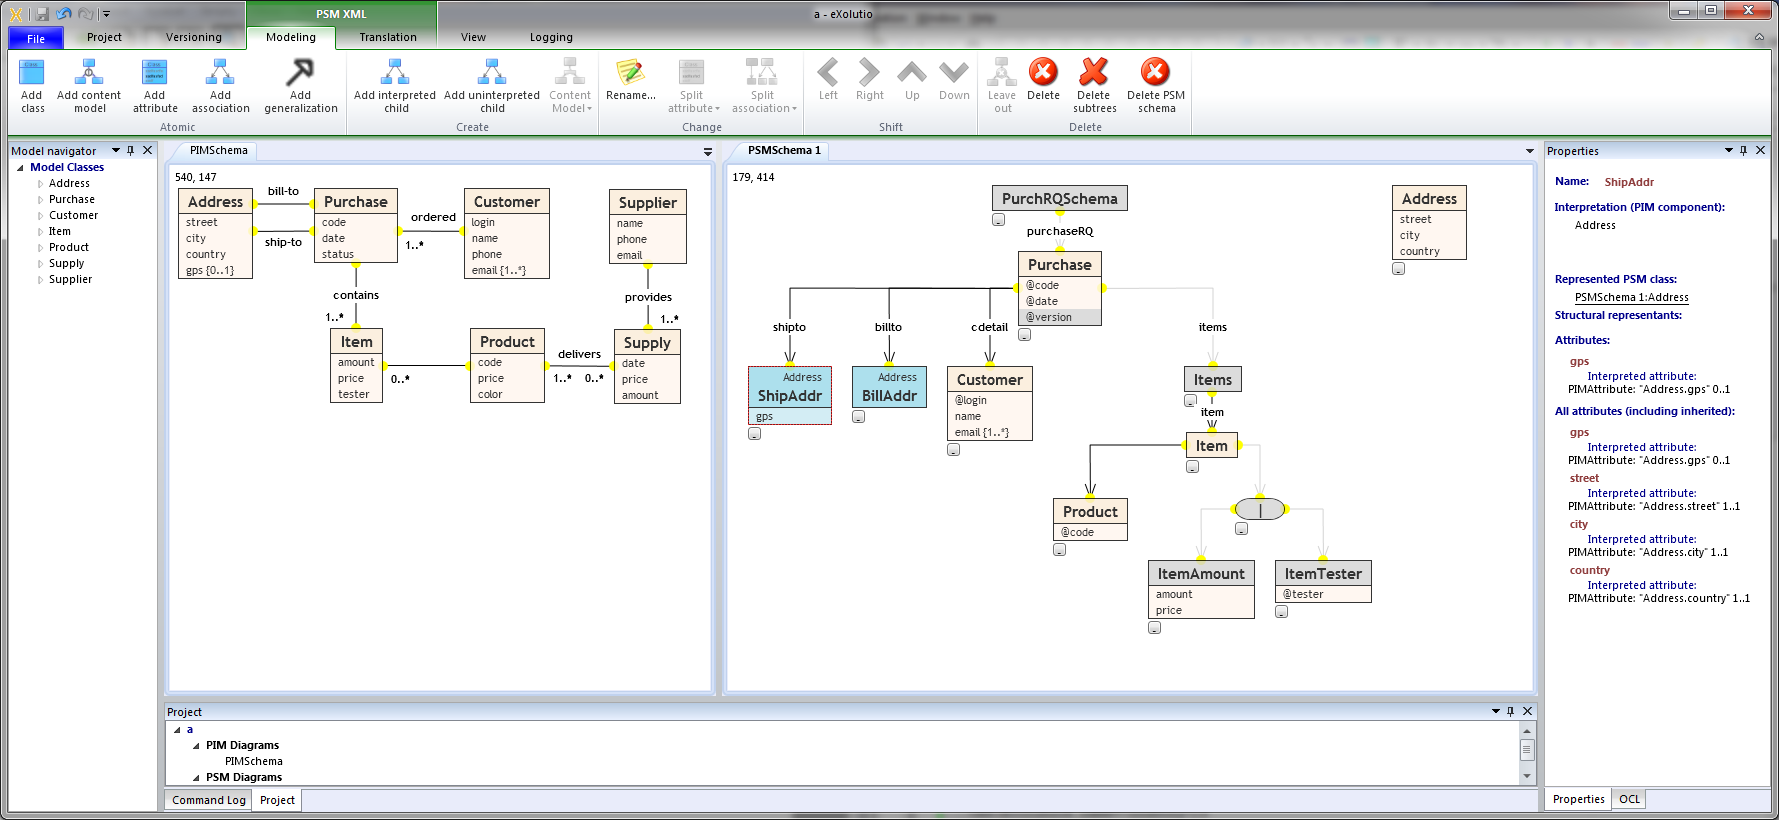
\includegraphics[width=\textwidth]{img/exolutio.png}
    \caption{Preview of the eXolutio tool. The left panel shows the PIM model as a UML class diagram, while the right panel represents a PSM schema in a tree-like structure that can be converted to an XML schema.}
    \label{fig:exolutio}
\end{figure}

Their primary use case was to create schemas for the government, such as the information system for National Register for Public Procurement (NRPP) for publishing public contracts.

\paragraph{Modeling} To create a schema, a user has to first create an ontology of desired entities as PIM. Then, multiple schemas can be created as PSM trees by first selecting a schema root and then adding entities to it. The resulting XML schemas then can be exported from the application.

\paragraph{Evolution of schemas} The focus of XRG was also directed to the evolution \cite{nevcasky2012evolution} of their proposed model to minimize the work of the data designer. As already stated in the introduction of the thesis, changes may be inevitable (either from the user requirements or from the surrounding environment) in large and complex systems, and propagating even a tiny change from the domain ontology to all affected schemas is time-consuming and error-prone.

They proposed, formalized, and later implemented a solution in restricting the changes in PIM and PSM models to only atomic operations - simple changes in the model, such as \textit{creating a new class}, \textit{updating a name of association} or \textit{removing an attribute}. Those operations are not intended to be used by the user directly but are simple enough to be formally defined and mapped to the corresponding operations in the level below. The proposed mapping is then used to propagate changes in the model to the schema level, more precisely from PSM to PIM, which is then translated to the schema level. They implemented only top-down propagation of changes as the propagation from XML documents is usually not meaningful (but theoretically possible).

\paragraph{Implementation} Their result were implemented in two tools \textit{XCase} \cite{xcase} and \textit{eXolutio} \cite{exolutio}. The former one was simpler, focused only on modeling. The latter then supported schema evolution as described in the previous section. Tools let users define the ontology from which the schemas and operations were derived for XML documents.

\paragraph{Analysis} The tool was designed only for XML, hence is not usable for other languages, such as JSON, which is very popular at the time of writing this thesis as being used by many server-centered applications to communicate with the server through the REST API \cite{fielding2000architectural}, for no-SQL databases\footnote{\url{https://www.mongodb.com/}}\footnote{\url{https://rethinkdb.com/}} and more. Nevertheless, we can use their findings and generalize the model for other formats.

They focused on the correctness and completeness of the model, which in some cases may be a limitation, such as more complex implementation and processing of the model to not allow a user to create a schema that is not valid.

Lastly, the tools didn't support sharing and collaboration, as at that time this was not considered standard practice in the industry.
\chapter{Requirement analysis}\label{chapters:analysis}

This chapter summarizes the expectations for the application in the form of requirements. The requirements are analyzed, and in the following chapter, the solution is proposed with a focus on a formal description of the framework.

\bigskip

As \textbf{stakeholders} we would consider data analysts, programmers, or at least people interested in the area of data modeling, since the typical use case of the application is (i) to design schemas for a large system of interconnected subsystems or modules, or (ii) to design a recommendation for publishing data. Both these use-cases were described in the introduction of this chapter.

Because of the stakeholders' knowledge in the area of data modeling, we may keep the UI of the application more technical as the intent of all operations may be intuitive for them. Nevertheless, the basic functionality does not require advanced knowledge in the mentioned fields, so we propose an "expert mode." The user will be asked whether he or she feels to be an expert in the area, which would make available more advanced features of the application while keeping the UI simple for those interested in the basics of data modeling.

\bigskip

\section{General schema}

\begin{requirement}
A user shall be able to easily derive a \textbf{general schema} structure from the existing ontologies and then translate the structure into different known schema languages, such as JSON Schema, XSD and CSVW Schema and it shall be possible to add support for others easily.
\label{requirement:general-schema}
\end{requirement}

The basic idea behind this requirement was already explained in the introduction chapter. From an ontology, which specifies the relations between things from a real world, it should be possible to easily select relations and things that will describe a schema. The schema then describes a structure of data that represents those things.

\begin{figure}[h!]\centering
  \begin{tikzpicture}
      %Nodes
      \node[ontology] (ontology) at (0,0) {Ontology};

      \node[general-schema] (schema1) at (-3.5,-1.5) {General schema 1};
      \node (psmDot) at (0,-1.5) {...};
      \node[general-schema] (schemaN) at (3.5,-1.5) {General schema N};

      \node[schema,align=center] (xml1) at (-5.5,-3) {XML\\schema};
      \node[schema,align=center] (json1) at (-3.5,-3) {JSON\\schema};
      \node[schema,align=center] (csv1) at (-1.5,-3) {CSV\\schema};

      \node (psmDot) at (0,-3) {...};

      \node[schema,align=center] (xmlN) at (1.5,-3) {XML\\schema};
      \node[schema,align=center] (jsonN) at (3.5,-3) {JSON\\schema};
      \node[schema,align=center] (csvN) at (5.5,-3) {CSV\\schema};

      %Lines
      \draw[-latex] (ontology) -- (schema1);
      \draw[-latex] (ontology) -- (schemaN);

      \draw[-latex] (schema1) -- (xml1);
      \draw[-latex] (schema1) -- (json1);
      \draw[-latex] (schema1) -- (csv1);

      \draw[-latex] (schemaN) -- (xmlN);
      \draw[-latex] (schemaN) -- (jsonN);
      \draw[-latex] (schemaN) -- (csvN);
  \end{tikzpicture}
  \caption{Diagram showing the core workflow behind the data modelling from an ontology. User can create general schemas (blue rectangles) from the ontology from which are created traditional data schemas, such as XSD, CSV Schema or JSON schema.}
\end{figure}

\smallskip

We aim to design a model for a general schema that can describe most of the serialization data formats. This model will be used as a mapping from the ontology to the desired schema. The model must be robust enough to support different formats, as we want to use the same for all of them.

There are many formats for data exchange, the most famous being JSON, XML, CSV/TSV, and RDF. The formats can be categorized into the following categories based on the model of the structure:
\begin{itemize}
    \item \textbf{Hiearchical model} stores data in a tree-like structure, having one root thing with properties that may recursively contain other things. It was one of the most common models for data serialization in the past few decades as it was easy to understand and interpret. XML and JSON are examples of formats that use this model.
    \item \textbf{Relational model} uses a set of tables to store data. Each table represents a sequence of similar things, each on one row with columns as properties. Rows may point to rows in other tables to link data. The relational model is also famous for its simplicity in CSV and TSV files which can be easily parsed.
    \item \textbf{Graph model} represents data in general graph structure with nodes and edges. RDF (Resource Description Framework) became a popular format using the graph model, where nodes usually represent things or literal values and edges connect them as properties.
\end{itemize}

As our primary intent is to support JSON and XML, we will use the first type of model to represent data in our general format. The translation from that format to individual schemas in the hiearchical model would be implicit.

Supporting translation from the general schema, which is in the hierarchical model, to the formats in the relational and graph models should be possible in a limited way\footnote{That means we may not be able to reverse translation from specific schema to the general schema or it may not be possible to use the full power of the given specific schema. However, this is not important to us as our target is support for basic use-cases.}, which is sufficient and follows the requirement to have one general schema.

The graph model is not even necessary to generate as we use the ontology that is already in the graph model; hence we can use the ontology directly as the schema to validate our data.


%==============================================================================%
\subsection{Analysis of the formats}

We will analyze the standard formats to properly design a user interface for the schema modeling and the underlying general schema model capable of describing those formats.

\smallskip

\textbf{JSON (JavaScript Object Notation)} is a simple format with two complex data types: objects and arrays. The objects represent data in key-value pairs, with values that can have any type, including other objects and arrays. Arrays then represent lists, and both arrays as objects may be in the root of the document tree. Semantically, objects represent things, with their values as properties.

\textbf{XML (Extensible Markup Language)} is similar to JSON as both formats are hierarchical. XML tags wrap parts of the document representing either things or properties of things and can be nested similarly to the JSON format. In contrast to JSON, XML tags can have attributes.

\begin{figure}[h!]\centering
    \begin{subfigure}[b]{.45\textwidth}
\begin{Verbatim}[commandchars=\\\{\}]
\{
  "id": 3758,
  "title": "Chair",
  "variants": [
    \{
      "title": "Black",
      "price": 200,
      "color": "black"
    \},
    \{
      "title": "White",
      "price": 200,
      "color": "white"
    \}
  ]
\}
\end{Verbatim}
        \caption{JSON document - braces {\tt\{\}} wraps object and brackets {\tt[]} wraps array}
      \end{subfigure}\hfil%
      \begin{subfigure}[b]{.45\textwidth}
\begin{Verbatim}[commandchars=\\\{\}]
<Good id="3758">
  <title>Chair</title>
  <Variant>
    <title>Black</title>
    <price>200</price>
    <color>black</color>
  </Variant>
  <Variant>
    <title>White</title>
    <price>200</price>
    <color>white</color>
  </Variant>
</Good>
\end{Verbatim}

\vfill

        \caption{XML document - {\tt<Good>} tag serves as a class wrapper, whether {\tt<title>} has a property meaning}
      \end{subfigure}
    \caption{Comparison of JSON and XML format both showing data about the same chair.}
    \label{analysis/xml-json}
\end{figure}

As seen from \autoref{analysis/xml-json}, the XML format is more complex, as it supports tag attributes (see the \verb|id="3758"| attribute), and arrays can be written in two distinct ways. We can place items of the array directly in the parent container, as we can see with the \verb|<Variant>| tag, or we can wrap them into another container for clarity (for example, into \verb|<variants>| tag).

\smallskip

JSON Schema is a JSON document describing the data structure we can expect in JSON documents. For this part of the thesis, it is sufficient to know that the schema defines which root object we can expect and a set of allowed properties and their types for each object.

Suppose we have chosen a structure very similar to JSON Schema to be our general structure format. We are interested only in how it describes the document's structure, not its representation. Because JSON is simpler than XML, we can use our model to describe only simple XML documents as we are missing constructs that would describe advanced XML features.

For example,
object property {\tt x} with primitive value {\tt y} would represent an XML tag {\tt <x>y</x>}; if {\tt y} is an object, we will recursivelly apply this rule.
Object property {\tt x} with an array of {\tt y\textsubscript{i}}  would represent multiple XML tags {\tt<x>y\textsubscript{1}</x><x>\nobreak\hfil\penalty0 \hfilneg y\textsubscript{2}</x>...<x>y\textsubscript{n}</x>}.
Finally, we will start with the root tag, which was {\tt <Good>} in our case.

To describe and distinguish between more advanced XML features, we would need to add XML-specific options to our model, such as:
\begin{enumerate}
  \item For every object property with a primitive value, there should be an option that the given property become an attribute of the parent tag. For example, the \verb|id| property of the chair may be either the attribute \verb|id="3758"| of the parent, or the full tag \verb|<id>3758</id>| inside the parent.
  \item For every array property, there should be an option that the given list of tags will be wrapped.
  \item XML, compared to JSON, recognizes an order of the elements in the document. This means that we may decide whether we want to enforce the specific order or not, which can also be fixed by another option in the parent.
\end{enumerate}

Comparing structure of JSON and XML once again, we can let a user use the JSON Schema-like structure with optional annotations for advanced XML features. This allows us to have a simple model which is easy to understand and use and can be annotated by other options for specific languages, as we have shown for XML.

\smallskip

\textbf{CSV (Comma-Separated Values)} or TSV stores data in tables. This, unfortunately, means that the structure is completely different than in the case of JSON and XML. Because having a separate schema would cause complications against other requirements, we will analyze whether it is possible to translate our general structure format from a hierarchical model to a relational one.

In the general case, there are existing approaches \cite{10.1145/304181.304220, 10.1007/3-540-45271-0_10} to map hierarchical model to relational. Therefore, we will show only a brief example. Suppose our general structure format contains objects, properties, and arrays. From each object type, we will create a table with columns as properties. Each table must have a primary key so that the tables can be linked together. If the schema contains an array, we will link children to the parent table; thus, array properties will not have a column.

\begin{figure}[h!]\centering
  \begin{subfigure}{.5\textwidth}
    \centering
    \begin{tabular}{ll}\toprule
      id   & title \\ \midrule
      3758 & Chair \\ \bottomrule
    \end{tabular}%
  \end{subfigure}%
  \begin{subfigure}{.5\textwidth}
    \centering
    \begin{tabular}{llll}\toprule
      good-id & title & price & color \\ \midrule
      3758 & Black & 200 & black \\
      3758 & White & 200 & white \\ \bottomrule
    \end{tabular}
  \end{subfigure}
  \caption{Document of two CSV tables representing the same data as in the \autoref{analysis/xml-json}. Left table contains the root.}
  \label{analysis/csv}
\end{figure}

Because all the tables represent arrays, we can not formally convert the schema with an object in the root. We have suppressed this in the \autoref{analysis/csv} simply by wrapping the schema root into the array.

To support CSV documents containing unrelated data, specifically CSV tables, that do not reference each other, we may need to have a schema with multiple roots. Multiple root schemas may be helpful in some advanced data-modeling problems. We will keep the question behind this open as there are not enough use-cases right now.

Although we have not dealt with advanced cases, the model is robust enough for most use cases.

\subsection{Designing the model}

So far, we have shown that a JSON Schema-like model with format-specific annotations is sufficient for describing a structure of JSON, XML, and CSV documents. In general, we cannot have too strict requirements on the model as some other formats may not require all the information or may be too simple. This pushes us to define the schema in the most elementary way.

\medskip

We will allow only classes to be a root of schemas and instead add an option that the root can be an array. This simplifies the work with the model as we may always expect a class.

Classes then have an ordered list of properties. This is different from JSON, where properties have no order. A property may be an attribute or association. An attribute has a primitive type, such as a string or a number. Association is a property with another class. Because we have forbidden the use of arrays in the root, we omit them entirely as an array of primitive values and classes can be achieved by the cardinality of attributes and associations, respectively. Cardinality is an interval specifying how many values a property can have. $1..1$ is for required properties, $0..1$ for optional, and $0..*$ for arrays.

\smallskip

We can use two different approaches to visualize the model's hierarchical structure. Previous tools \textit{xCase} and \textit{eXolutio} used graph visualization, where nodes were used to show classes and edges to show associations. An alternative approach is to use a textual "bullet list" representation, as the model is \textit{usually} a tree.

The latter approach is easier to understand as the final product is a schema for documents that has a similar "structure" as the representation. It is easier to implement, more compact in size on the screen, and easier to work with on smaller devices. Also, the order of the properties is more intuitive, and we can use more styling options for advanced constructs.\footnote{So far, we have described only a basic schema structure. See other requirements for advanced constructs.} However, in the general case, users may benefit from the graph view if the schema refers to another schema (see the \autoref{analysis/requirement/schema-reference}) multiple times because this can be easily denoted in the graphical interface (see \autoref{analysis/difference-between-graphical-and-hiearchical}).

\begin{figure}[h!]\centering
  \begin{subfigure}{.5\textwidth}
      \centering
      \begin{tikzpicture}[
          squarednode/.style={rectangle, draw=blue!60, fill=blue!5, very thick, minimum size=5mm},
      ]
          %Nodes
          \node[ontology] (root) at (0,0) {root class};

          \node[squarednode] (a1) at (-1.5,-1.5) {association 1};
          \node[squarednode] (a2) at (1.5,-1.5) {association 2};

          \node[ontology] (ref) at (0,-3) {referenced class};

          %Lines
          \draw[-latex] (root) -- (a1);
          \draw[-latex] (root) -- (a2);
          \draw[-latex] (a1) -- (ref);
          \draw[-latex] (a2) -- (ref);
      \end{tikzpicture}
      \caption{Graphical representation}
    \end{subfigure}%
    \begin{subfigure}{.5\textwidth}
\begin{Verbatim}[commandchars=\\\{\}]
{\color{purple!60}root class}
  {\color{blue!60}- association 1} to
      {\color{purple!60}referenced class}
  {\color{blue!60}- association 2} to
      {\color{purple!60}referenced class}
\end{Verbatim}
      \caption{Hiearchical representation}
    \end{subfigure}

  \caption{Figure showing a schema referencing the same subschema twice, essencially creating a cycle in unoriented graph. Two different representations are shown - graph and hiearchical.  The former one shows that both associations refer the same subschema, which later representation can not show.}
  \label{analysis/difference-between-graphical-and-hiearchical}
\end{figure}

Because the main use-case is to generate simple or moderately advanced schemas, the textual approach is preferred. Nevertheless, the graph view might be implemented in the future.

\medskip

As shown in the \autoref{analysis/difference-between-graphical-and-hiearchical}, the schema may be represented as a "bullet list" where each class, association, or attribute is on a separate line. Classes have a list of properties under the class name. Associations point directly to other classes, and, therefore, they can be merged with the class name on a single line. Other attributes, including format-specific, will be on the line next to the item name.

\begin{figure}[h!]\centering
  \begin{Verbatim}[commandchars=\\\{\}]
{\color{purple!60}class \textbf{Good}}
  {\color{blue!60}- attribute \textbf{id}}[1..1]: string
  {\color{blue!60}- attribute \textbf{title}}[1..1]: string
  {\color{purple!60}- association \textbf{variants}}[0..*]: \textbf{Variant}
    {\color{blue!60}- attribute \textbf{title}}[1..1]: string
    {\color{blue!60}- attribute \textbf{price}}[1..1]: number
    {\color{blue!60}- attribute \textbf{color}}[1..1]: string
\end{Verbatim}
  \caption{Proposition for how the general schema may be represented for the example that validates data with the chair.}
  \label{analysis/general-schema-representation}
\end{figure}

It shall be possible to change the order of the properties by dragging them, and options for given items shall be available next to them. Attributes and associations shall be distinguished both by color and supporting graphics. More advanced constructs may have unique styling options to provide more information if necessary.

\section{Ontology}

\begin{requirement}
    \label{requirement:ontologies-on-the-web}
    As many ontologies are located on the web in formats such as OWL (Web Ontology Language), RDFs (RDF Schema), UFO (Unified Foundational Ontology), etc., the application shall support reading them.
\end{requirement}

It may seem that designing the ontology directly in the tool is beneficial because a user does not need to use other tools and the application may already build the schema, which is a feedback to the user. This approach was used in tools \textit{XCase} and \textit{eXolutio} as can be seen in the \autoref{fig:exolutio} in the left panel. However, it has the following drawbacks:

\begin{enumerate}
    \item Designing an ontology is a well-defined problem. There are many great and time-proven tools we could not cope with.
    \item Even if the ontology will be used just to generate the schemas, it may be worthy of publishing it anyways as others may benefit from it.
    \item It is better to split a complex problem into smaller ones.
\end{enumerate}

On the other hand, not having direct access to the ontology, as it will be on the Web, has the following impacts:

\begin{enumerate}
    \item The ontology may \textbf{not always be available}. Unavailability should not prevent us from generating the schemas and making minor changes to them if those changes are not directly related to exploring the ontology.
    \item The concepts in the ontology may \textbf{point to another ontology} according to the Linked Data principles.
\end{enumerate}

For the reasons mentioned above, the preferred workflow is to design the ontology separately in the external tool, publish it on the Web, and then model the schema in the application. There is \autoref{requirement:pim-editing} later in the text specifying that a user can make modifications in the application. This is not inconsistent with the statements, as it deals with minor changes instead of defining a complete ontology.

The term ontology has already been defined in the introductory chapter, and we will formally define its specific requirements in the next chapter.

It shall be easy to implement support for other types of ontologies, and all of them shall be linkable according to the LD principles.

\subsection{Format of the ontology}

In the above requirement, several different formats were proposed for the ontology. This section will analyze the minimal requirements for any ontology format and how we will treat additional information in them. Because the core goal is to design schemas, we will start with a model proposed from \autoref{requirement:general-schema}. The schema consists of classes and their properties. A class corresponds to a thing from real life. An attribute is a literal that belongs to the given class only. On the other hand, an association is a link between two (not necessarily different) classes. From this point of view, the association is an independent entity.

Associations are usually oriented, and some ontologies may specify a title and a description for a reverse direction. For example, in RDFS, the association (or property in the RDFS terminology) is an entity of type {\tt rdf:Property} having domain and range classes and a title and description. Therefore, it only describes the forward direction. We can, of course, create a property in the other direction as well, but there would not be a connection between a forward and a reverse direction. Hence, we would not know that those are semantically the same properties. UFO (Unified Foundational Ontology), as an example of a more complex ontology, introduces relators. Relators are relationships between two or more things connected by mediation. The mediation can be described, giving us a way to describe both directions differently.

Although the latter approach is more complex, using simple concepts for associations may be disadvantageous for the aforementioned reason. Therefore, we will follow the pattern of UFO and any other simpler ontologies, such as RDFS, will not have the reverse direction described.

\medskip

An ontology in the context of this requirement is a set of classes that have attributes. The associations then connect two classes together. The connected classes may not have the same ontology.

As some formats specify the ontology in a more complex way, the application may use the additional information to better design the schema. This statement is better defined in the next chapter.

\begin{figure}[h!]\centering
  \centering
  \begin{tikzpicture}[
    attribute/.style={align=center},
  ]
    \node[ontologyClass] (good) at (0,0) {<<class>>\\\textbf{Good}};
    \node[ontologyClass] (variant) at (9,0) {<<class>>\\\textbf{Good variant}};

    \node[attribute] (a11) at (-.75,1.5) {<<attr>>\\id};
    \node[attribute] (a12) at (.75,1.5) {<<attr>>\\title};

    \node[attribute] (a21) at (7.5,1.5) {<<attr>>\\title};
    \node[attribute] (a22) at (9,1.5) {<<attr>>\\price};
    \node[attribute] (a23) at (10.5,1.5) {<<attr>>\\color};

    \draw (good) -- (a11);
    \draw (good) -- (a12);

    \draw (variant) -- (a21);
    \draw (variant) -- (a22);
    \draw (variant) -- (a23);

    \draw (good) -- node[pos=0.225,below]{$\blacktriangleleft$ is variant of} node[above]{<<association>>} node[pos=0.775,below]{has variant $\blacktriangleright$} (variant);
  \end{tikzpicture}

  \caption{Schematic diagram of an ontology which could be used for the schema from the \autoref{analysis/general-schema-representation}.}
  \label{figure:example-of-ontology}
\end{figure}

% todo popis, jak by mela ontologie vypadat na zaklade toho schematu. Jakou by mela mit strukturu a co musi obsahovat

% mozna ze to je jak uml

\section{Data modeling analysis}

\subsection{Type coherency}\label{subsection:type-coherency}

As already mentioned, an ontology is not just a supporting source for the modeling process but rather the only source we can use to create schemas. The schema then represents a mapping to the ontology for further processing.

Because parts of the schema are mapped, we can check whether the attributes and associations belong to the given class. This allows us to check whether the schema is being built correctly and to provide the appropriate help during the modeling based on the type of the classes.

Although the problem may seem trivial, there are advanced scenarios that must be considered.

\begin{enumerate}
  \item We may want to add additional attributes and associations directly into the schema without a connection to the ontology. This is a schema-modeling problem as we may need, for example, to wrap several properties into an additional object (JSON) or a tag (XML) or add another property because the data we validate contains it.
  \item If $A$ is associated with $B$ and we have a schema with the class $A$ having $B$, then it may be possible to move attributes\footnote{Moving of properties to different classes will be kept as future work. Nevertheless, to cover some use cases, we employ a simpler construct of dematerialization. Association that is dematerialized is removed from the generated result and all properties from the associated class are moved on its place.} from $A$ into $B$. Because for each $B$, we know to which $A$ it belongs, we do not lose any information during this process.
\end{enumerate}

As an example of the second case, suppose that our ontology has \textit{Goods} and their \textit{Variants}. Variants are colors, sizes, and materials for the given item. Indeed, all variants are made by one manufacturer. Therefore, it makes sense that the \textit{manufacturer} attribute would be associated with the \textit{Goods} class, whether the \textit{color} with the \textit{Variants}. This may not be a beneficiary for all data consumers. Therefore, a schema with the \textit{manufacturer} attribute moved into the \textit{Variants} class might be a better solution.

\begin{figure}[h!]\centering
  \begin{subfigure}[b]{.5\textwidth}
    \begin{Verbatim}[commandchars=\\\{\}]
\{
  "title": "Chair",
  "variants": [
    \{
      "price": 200,
      "color": "black",
      \textbf{"manufacturer": "IKEA"}
    \}
  ]
\}
    \end{Verbatim}
  \end{subfigure}%
  \begin{subfigure}[b]{.5\textwidth}
    \begin{Verbatim}[commandchars=\\\{\}]
\{
  "customerId": "12",
  {\color{gray!60}"personal-info": \{}
    "name": "John",
    "surname": "Doe"
  {\color{gray!60}\},}
  {\color{gray!60}"contact-info": \{}
    "address": ...,
    "phone": ...
  {\color{gray!60}\}}
\}
    \end{Verbatim}
    \end{subfigure}%
  \caption{Examples of data with some attributes moved. The former moves the attribute \textit{manufacturer} from the parent into the other class that has a counterpart in the ontology. The latter takes attributes such as \textit{name} and \textit{address} and wraps them with additional objects that do not correspond to the ontology.}
\end{figure}

However, this is too complex for the current state of development, but it gives us a chance to think about the problem in a more general way.

\subsection{Data modeling process}

So far, we have only described the desired structure of an ontology and a schema model, but we did not tackle the actual process of how the schema is created.

A user starts by selecting a root of the schema. Schema under the given root would then describe one entity of the given type, or a list of those entities, depending on the later configuration. Because a set of possible root classes is not limited in any way (or, we can say that the root has the most general type, hence can be specialized), the most suitable option is to let the user search for the class by its name, descriptions, or other parameters, depending on the given ontology format.

As soon as the root is placed in the schema, we get a context because the following attributes and associations to other classes depend on the class where the properties are being added. For that, we use a prompt dialog where it is possible to select those properties to be added.

Although we did not enforce that an ontology must support inheritance, most of them do. Therefore, the dialog also allows adding properties of the parent class.

\medskip

The process of adding properties can be more automated in the future. The tool can propose to automatically add all attributes and associations with nonzero cardinality, as it may be the desired behavior. We can perform this action even recursively to automatically design the whole schema just from the root and select a few options where the recursion shall stop.

In general, there might be cases with hundreds of available entities to add where only some of them are relevant to the current user. This is further supported by the fact that anyone can extend our ontology by introducing their classes associated with ours. To properly understand the relevance of different entities, a user profile from past choices needs to be built. This is an area of recommended systems, with many focusing specifically on model-driven engineering \cite{almonte2022recommender}, and we will consider them in our future work. % not a requirement

\bigskip

\begin{requirement}
    The application shall create supporting documents for the generated schemas.
\end{requirement}

The main goal of the tool is to model schemas from a given ontology. Nevertheless, to better understand the generated schema, the documentation, possibly with diagrams and examples, is very beneficial.

A structure of the documentation was already described in the introductory chapter and can be easily derived, as it only describes used concepts that are mapped from the schema.

Regarding examples, for the schema in \autoref{analysis/general-schema-representation}, Figures \ref{analysis/xml-json} and \ref{analysis/csv} could be automatically generated. This would require additional knowledge from the ontology as the application needs to understand that the title should be a buyable item (hence \textit{chair} and not \textit{sitting} for example) and the price should be reasonable to the item's actual price (because it may confuse users when the price would too low or too high).

\section{Data transformations}

\begin{requirement}
    The application shall support generating transformations between different data conforming to supported schemas and RDF representation.
    \label{req:transformations}
\end{requirement}

Data transformations were also introduced at the beginning of this thesis. In general, \textbf{data transformations} are used to convert data (not schemas, but data that conform to given schemas) from one schema to another without changing its meaning.

One example may be to convert CSV to a JSON array of objects, where each object represents a row in the CSV. There are plenty of online tools to do this, but they do not understand the context of the data. Because both schemas were designed in the tool, we may exploit the knowledge of the mapping to the original ontology and correctly map columns from CSV to the fields in a JSON object.

In the context of this tool, transformation means both (i) transformation between different schemas under the same general schema and (ii) between different general schemas, if possible. As an example of the second case, we may have two general schemas for the same thing, where one is simpler than the other. For example, we may have the schema from \autoref{analysis/general-schema-representation} and similar with more attributes and associations, possibly with a different order of properties and labels. It is then possible to convert the data from the more complex schema to the simpler one by loosing the information. If default values are provided, or additional properties are optional, the transformation in the other direction should also be possible.

\medskip

Regarding the transformation process, there are plenty of ways to transform the data:
\begin{enumerate}
    \item Data engineers use \textbf{Python} with support for many formats using libraries. In this case, the transformation would mean a generated Python script with a predefined interface that takes data from one format and outputs in another. Depending on the use case, the script may be configurable (besides the possibility to configure the generation of transformation itself).
    \item There is \textbf{XSLT} (Extensible Stylesheet Language Transformations) language to transform between XML documents or from XML to XML-like, plain-text, or CSV documents. XSLT is an XML document that can be executed with an input document by an XSLT processor, producing the resulting document. A disadvantage is that the input document must be in XML format; hence, it cannot be used alone for bidirectional JSON and CSV transformation.
    \item There are mapping tools and languages, such as \textbf{RML} \cite{dimou2014rml} (RDF Mapping Language) designed explicitly for mapping purposes. RML maps common serialization frameworks, such as XML, CSV, and JSON, to RDF from a set of rules written in RDF. The translation mechanism is similar to the XSLT. Specifically for JSON, there is \textbf{JSON-LD} with simple rules to set mapping to RDF. Conversion tools are available in multiple programming languages.
\end{enumerate}

Although RML is a ready-to-use solution with support for all three technologies, it requires its own transformation toolchain. On the contrary, XSLT is a well-known technology among people working with XML and is widely supported. Our primary goal is to have transformations that are easy for stakeholders to use in their systems. Therefore, we will implement XSLT for XML while keeping RML for later.

Similar to the translation of a human text, there are two approaches. Either create a transformation for each pair, or have one standard format where all the others can be transformed and vice versa. The latter approach requires only one transformation for each new format added and is easier to debug, as there is a middle format. Because schemas are built from ontologies whose primary source is RDF, we will exploit this and have RDF as the middle format, which is another format to which we can transform data.

\medskip

We categorize two types of transformation, lifting and lowering. Lifting is a process of converting semi-structured data such as JSON, XML, or CSV into RDF. Lowering is the opposite process. By combining them, we can achieve a transformation between various formats. That means that even if we want to transform XML to CSV, which would be possible by a single XSLT document for simple structures, we would need to execute two transfomations.

\begin{figure}[h!]\centering
    \begin{tikzpicture}
        %Nodes
        \node[ontology] (ontology) at (0,0) {Ontology};

        \node[artefact,align=center] (rdf) at (3,-1.5) {RDF documents};

        \node[general-schema,align=center] (schema1) at (-3,-1.5) {General\\schema};

        \node[schema,align=center] (xml1) at (-4,-3) {XML\\schema};
        \node[schema,align=center] (json1) at (-2,-3) {JSON\\schema};

        \node[artefact,align=center] (xml_document) at (1.5,-3.5) {XML\\document};
        \node[artefact,align=center] (json_document) at (4.5,-3.5) {JSON\\document};

        \draw[-latex] (rdf) -- node[above,anchor=south west,align=left] {conforms} (ontology);

        \draw[-latex] (ontology) -- (schema1);
        \draw[-latex] (schema1) -- (xml1);
        \draw[-latex] (schema1) -- (json1);
        \draw[-latex] (xml_document) to[bend left] node[below] {conforms} (xml1);
        \draw[-latex] (json_document) to[bend left] node[below] {conforms} (json1);

        \draw [->,line width=1pt, transform canvas={xshift=-1.25em}] (xml_document) -- (rdf);
        \draw [->,line width=1pt, transform canvas={xshift=-0.5em}] (rdf) -- (xml_document);

        \draw [->,line width=1pt, transform canvas={xshift=0.5em}] (json_document) -- (rdf);
        \draw [->,line width=1pt, transform canvas={xshift=1.25em}] (rdf) -- (json_document);

        \node[rectangle,fill=white] at (3,-2.35) {lifting and lowering};
    \end{tikzpicture}
    \caption{Example of data transformation. An XML document that conforms to XML schema may be lifted to RDF representation, which conforms to the ontology. The RDF can then be lowered to another format.}
\end{figure}

\section{Data specification}

The following requirements force us to group similar general schemas into a project that we call a \textbf{data specification}. Schemas in the data specification may share some configuration or depend on each other, as we specify later. Each schema belongs to exactly one data specification. We will not determine in this thesis which schemas should share a data specification and which should not because there are currently no limitations that would state otherwise. However, this may change in the future as new requirements arise.

\begin{requirement}
  It shall be possible to refer to other schemas to use them as building blocks for larger ones. Schema reference shall be treated as a reference to the resulting schemas and documentation as well.
  \label{analysis/requirement/schema-reference}
\end{requirement}

Referencing other schemas is crucial for advanced use cases where it is essential to split large schemas into smaller blocks that can be published and used separately.

For most schema languages, it should be sufficient to refer to the other schema as is. For example, in JSON, we can use the \verb|$ref| keyword with a path to the referenced schema. On the other hand, data transformations may not always be able to handle this approach. Hence, having a full copy of the schema might be necessary. Referencing a schema would thus require access to all data in its specification.

To avoid problems with tracking references and knowing which data specification needs to be loaded to generate artifacts properly, a user would need to explicitly set a given \textbf{data specification is being reused}. Similarly to the requirement with the ontology, we do not require that the reused data specification be always available.\footnote{See the requirement X for context.} The application shall work even if the data specification is not available at the moment if the presence of the specification is not required directly, such as for creating a new reference or generating artifacts that depend on it.

\begin{figure}[h!]\centering
  \begin{tikzpicture}
      \node[dataSpecification,align=center] (ds1) at (-3,0) {Data specification 1};
      \node[dataSpecification,align=center] (ds2) at (3,0) {Data specification 2};

      \node[generalSchema,align=center] (s11) at (-4.5,-1.5) {General\\schema};
      \node[generalSchema,align=center] (s12) at (-1.5,-1.5) {General\\schema};
      \node[generalSchema,align=center] (s21) at (3,-1.5) {General\\schema};

      \draw[-latex] (ds1) -- (s11);
      \draw[-latex] (ds1) -- (s12);
      \draw[-latex] (ds2) -- (s21);

      \draw[-latex,densely dotted] (ds1) -- node[above] {reuses} (ds2);
      \draw[-latex,densely dotted] (s12) -- node[above] {refers} (s21);
  \end{tikzpicture}
  \caption{Example of reusing of specifications. All schemas from reused specification become available to refer from local schemas. Only the root of the schema may be refered.}
\end{figure}

\begin{requirement}
  The list of supported schemas, transformations, documents, and other files generated from the general schema shall be easily expandable to adapt the tool to different use cases.
\end{requirement}

The generation of schemas is robust enough to be used in every common scenario. Therefore for most users, we do not expect they may want to intervene in the process besides the standard configuration, such as indentation, using of comments, or a default language.

On the other hand, documentation is a very vague concept that neither we have adequately specified. Sometimes simple Markdown documentation may be sufficient, while elsewhere, the user may require a strict format of multiple documents in HTML.

Transformations have similar issues. There are multiple ways and technologies that transform data between different schemas. We have already mentioned transformation through the RDF format, either by RML or custom scripts, such as XSLT for XML. For the more demanding user, it is even possible to create transformation scripts between pairs of different serialization formats, such as between XML and CSV.

We will expose a way the user can register their own generator that can create a set of files in a filesystem from the given schema.

To support the linking of generated files, generators may use others to modify their results, further expand them, or create a link to them. This is specifically useful for documentation, as it should contain links and possibly a copy of generated schema.

\subsection{Artifacts}

There is little difference between generated schemas, data transformations, documentation, and other output files. Based on the general schema and provided configuration, if any, the application shall create a set of files that can either be published on the Web or stored in the file system. All generated files will be denoted as \textbf{artifacts} and created by \textbf{generators}.

We will distinguish two types of artifacts. (i) \textbf{Specification artifacts} do not depend on a concrete schema but use the whole specification. Documentation may be an example of a specification artifact because it generates a single document concerning all schemas. Of course, schema-specific documentation is possible, and it purely depends on user requirements. (ii) The \textbf{schema artifacts} are bound to a concrete general schema and are used to generate transformations or schema documents.

\begin{figure}[h!]\centering
  \begin{tikzpicture}
      \node[dataSpecification,align=center] (ds1) at (-3,0) {Data specification};

      \node[generalSchema,align=center] (s11) at (-4.5,-1.5) {General\\schema};
      \node[generalSchema,align=center] (s12) at (-1.5,-1.5) {General\\schema};

      \node[schema,align=center,cascaded] (sa1) at (-7.5,-1.5) {Specification\\artefacts};

      \node[schema,align=center,cascaded] (sa11) at (-4.5,-3) {Schema\\artefacts};
      \node[schema,align=center,cascaded] (sa12) at (-1.5,-3) {Schema\\artefacts};

      \draw[-latex] (ds1) -- (s11);
      \draw[-latex] (ds1) -- (s12);
      \draw[-latex] (ds1) -- (sa1);

      \draw[-latex] (s11) -- (sa11);
      \draw[-latex] (s12) -- (sa12);
  \end{tikzpicture}
  \caption{Schemas, documentation, and other generated files are artifacts. Artifacts are either schema-specific, generated for every schema, or specification-specific for a given data specification.}
\end{figure}

% Necaskeho pozadavek na OR a hierarchii
% https://github.com/mff-uk/dataspecer/issues/95

% Zacnu tim, co vlastne chci a pak introducnu ten or
% neni to uz pak nahodou problem formalni analyzou

\section{Inheritance}

\begin{requirement}
    The tool shall support class inheritance on a general schema level and in generated schemas. That means it shall be possible to design a schema that validates data where both the base and derived classes can be used. The derived class may have additional properties.
    \label{requirement:inheritance}
\end{requirement}

\begin{showcase}
  We will start directly with an example. Suppose that the warehouse also distributes foods in addition to general goods. Food is a type of good, but it may have additional attributes for storage purposes, such as \textit{storing temperature} or \textit{expiration date}. Suppose that we want to design a schema for a JSON list of goods, as seen in \autoref{analysis:inheritance:json-data}. The document is an array of objects, where each object has basic properties such as \textit{name} and \textit{price}. If the object represents food, we want it to have the additional attributes. JSON Schema format is capable of supporting this.

  \begin{figure}[H]\centering
      \begin{Verbatim}[commandchars=\\\{\}]
[
  \{
    "name": "Chair",
    "price": 100,
    "type": "furniture"
  \},
  \{
    "name": "Ice-cream",
    "price": 10,
    "type": "food",
    "expirationDate": "2022-07-21",
    "storingTemperature": "frozen"
  \}
]
      \end{Verbatim}
      \caption{Example of JSON data we want to validate. Based on the type of good, the object may have additional properties.}
      \label{analysis:inheritance:json-data}
  \end{figure}

    Without any additional information, we can only say that if the object contains only one of those additional properties, it is not valid, because there is no such class that has only one of them. Nevertheless, we can add a property that specifies the type (or category) of goods and use this to validate the object.
\end{showcase}

This requirement impacts the application at three different levels. (i) The general schema model must have constructs representing the required problem. This is analyzed mainly in the following chapter. (ii) We must somehow represent the inheritance in the user interface. By this, we mean how to show that the class has a specialization in the "bullet list" representation (see \autoref{analysis/general-schema-representation}). (iii) All generators shall understand them and generate a schema that corresponds to the intended result.

\medskip

An advanced reader may point out that the problem can be generalized by introducing a disjunction to the schema. As we will show in the following text, this assumption is correct. Hovewer, designing schemas only with disjunction is a cumbersome and complicated task for less advanced users. Therefore, we still want to provide the ability to work more efficiently with the inheritance.

In ordinary cases, a more general class shares its properties with all its descendants. This can be seen in the example, where the \textit{Ice-cream} has all properties a \textit{Chair} has. In UML modeling and most programming languages, copying the properties is unnecessary as they are inherited. We want to achieve a similar thing in our schema representation, not polluting the page with redundant information. This, however, restricts the use of inheritance because we can not select the order of properties in the descendant class if the properties are not shown.

To formalize the restriction, a descendant class implicitly has all properties of the parent in the same order, and those properties are before any other properties of the descendant class. This is a limitation for XML and CSV documents as JSON does not depend on the order of properties. However, order generally does not play a huge role in modeling. For advanced use cases, the low-level constructs introduced later can be used.

The rule is applied through the whole chain of inheritance. If there are classes $A$, $B$, and $C$, where $C$ is a descendant of $B$ and $B$ is a descendant of $A$, then $C$ has properties of $A$, properties of $B$, and then its own properties.

In some situations, we might want to omit the parent class from a schema. Let us have a base class $B$ and its two descendants $M$ and $N$. So far, we can model a schema with either $B$, $M$, or $N$, where $B$ provides properties to both $M$ and $N$. $B$ may not represent a real thing per se. It may correspond to an abstract class that serves only as a base for the other classes. In that scenario, we only want to allow $M$ and $N$ to be used.

\medskip

Because we do not want to show inherited properties, the descendant classes must visually belong to their parent to understand that it shares its properties. Hence, we propose that if a class has a specialization in a schema, the specialization will be shown after the properties of the parent. If the base class should be omitted from the schema but has some properties, it will be shown visually differently.

\begin{figure}[h!]\centering
  \begin{Verbatim}[commandchars=\\\{\}]
{\color{purple!60}class \textbf{Good}}
  {\color{blue!60}- attribute \textbf{name}}[1..1]: string
  {\color{blue!60}- attribute \textbf{price}}[1..1]: number
  {\color{purple!60}specialization \textbf{Food}}
    {\color{blue!60}- attribute \textbf{expirationDate}}[1..1]: string
    {\color{blue!60}- attribute \textbf{storingTemperature}}[1..1]: number
    {\color{purple!60}specialization \textbf{Fruit and Vegetables}}
    ...
  {\color{purple!60}specialization \textbf{Drink}}
    ...
\end{Verbatim}
  \caption{Proposition for representing an inheritance in the schema. The row with specialization classes is below the property list and does not belong to it.}
\end{figure}

So far, the internal schema model, although not formally defined, does not support constructs for the purpose of inheritance. We can build on the current proposal of the UI, but this approach is not robust enough. We want to compose the desired results from low-level constructs.

\subsection{Disjunction in schemas}

First, we introduce the concept of a disjunction. The disjunction in a schema context is a set of rules (or subschemas) where exactly one rule must be satisfied. The disjunction serves as the "OR" operator in the schema. We can use it in our inheritance problem to create an association to a disjunction of classes that have a common ancestor. It nicely solves part of the inheritance problem and can be used for other things, as well. For example, the title can be either a string or an object of language and translation pairs.

Both the JSON Schema and the XML Schema support some kind of disjunction. JSON Schema has the {\tt anyOf} keyword, which specifies that the given value must match at least one rule, effectively creating an OR. XSD has {\tt xs:choice} element doing the similar thing.

There are two ways to implement the OR operator in our proposed hierarchical model: on a \textbf{class level} and \textbf{property level}. The former approach allows the OR operator to be placed anywhere where classes can be placed. Either in the root of the schema or in the association. The OR is then a set of classes. The latter approach is more flexible, allowing users to specify the disjunction between tuples of properties.

\begin{figure}[h!]\centering
  \begin{subfigure}[b]{.5\textwidth}
    \centering
    \begin{tikzpicture}[
      type-or/.style={diamond, draw=orange!60, fill=orange!5, very thick},
      type-class/.style={rectangle, draw=red!60, fill=red!5, very thick},
      type-attribute/.style={rectangle, draw=blue!60, fill=blue!5, very thick},
      level 1/.style = {sibling distance = 3.5cm, level distance = 1cm},
      level 2/.style = {sibling distance = 1cm, level distance = 1cm},
      every child/.style={-latex}
    ]
      \node[type-or] (root) {or}
        child {
          node[type-class] {$C^1$}
            child {node {...}}
            child {node[type-attribute] {$A_1$}}
            child {node {...}}
        }
        child {
          node[type-class] {$C^2$}
            child {node {...}}
            child {node[type-attribute] {$A_2$}}
            child {node[type-attribute] {$A_3$}}
            child {node {...}}
        };
      \draw[-latex] (0,1) -- (root);
    \end{tikzpicture}
    \caption{Class-level OR}
    \end{subfigure}%
    \begin{subfigure}[b]{.5\textwidth}
    \centering
    \begin{tikzpicture}[
      type-or/.style={diamond, draw=orange!60, fill=orange!5, very thick},
      type-class/.style={rectangle, draw=red!60, fill=red!5, very thick},
      type-attribute/.style={rectangle, draw=blue!60, fill=blue!5, very thick},
      type-or-group/.style={circle, draw=orange!60, fill=orange!5, very thick},
      level 1/.style = {sibling distance = 1.5cm, level distance = 1.125cm},
      level 2/.style = {sibling distance = 2cm, level distance = .5cm},
      level 3/.style = {sibling distance = 1cm, level distance = 0.75cm},
      every child/.style={-latex}
    ]
      \node[type-class] (root) {$C$}
        child {node {...}}
        child {
          node[type-or] {or}
            child {node[type-or-group]{} child{node[type-attribute] {$A_1$}}}
            child {node[type-or-group]{}
                child {node[type-attribute] {$A_2$}}
                child {node[type-attribute] {$A_3$}}
            }
        }
        child {node {...}};
      \draw[-latex] (0,1) -- (root);
    \end{tikzpicture}
    \caption{Property-level OR}
    \end{subfigure}%
  \caption{Comparison of two models of the semantically same subschemas of class $C$ having either attribute $A_1$, or both $A_2$ and $A_3$.}
\end{figure}

The former model is more common for programmers, as in some languages (such as TypeScript), it is possible to specify a type of property in this particular way as an OR of multiple types. On the other hand, the latter approach is more well known in data modeling, as XSD's {\tt xs:choice} works exactly the same way.

The model using a property-level OR can not use the disjunction in the root of the schema, which is an essential disadvantage as there may be use-cases for those schemas. On the other hand, this model is better suited for the Cartesian product of multiple disjunctions in a single class. Suppose a schema for class $C$ having the following attributes: the first attribute is either $A_11$ or $A_12$, and the second attribute is either $A_21$ or $A_22$.

\begin{figure}[h!]\centering
  \begin{subfigure}[b]{.6\textwidth}
    \centering
    \begin{tikzpicture}[
      type-or/.style={diamond, draw=orange!60, fill=orange!5, very thick},
      type-class/.style={rectangle, draw=red!60, fill=red!5, very thick},
      type-attribute/.style={rectangle, draw=blue!60, fill=blue!5, very thick},
      level 1/.style = {sibling distance = 2.2cm, level distance = 1cm},
      level 2/.style = {sibling distance = 1cm, level distance = 1cm},
      every child/.style={-latex}
    ]
      \node[type-or] (root) {or}
        child {
          node[type-class] {$C^1$}
            child {node[type-attribute] {$A_{11}^1$}}
            child {node[type-attribute] {$A_{21}^1$}}
        }
        child {
          node[type-class] {$C^2$}
            child {node[type-attribute] {$A_{11}^2$}}
            child {node[type-attribute] {$A_{22}^2$}}
        }
        child {
          node[type-class] {$C^3$}
            child {node[type-attribute] {$A_{12}^3$}}
            child {node[type-attribute] {$A_{21}^3$}}
        }
        child {
          node[type-class] {$C^4$}
            child {node[type-attribute] {$A_{12}^4$}}
            child {node[type-attribute] {$A_{22}^4$}}
        }
        ;
      \draw[-latex] (0,1) -- (root);
    \end{tikzpicture}
    \caption{Class-level OR}
    \end{subfigure}%
    \begin{subfigure}[b]{.4\textwidth}
    \centering
    \begin{tikzpicture}[
      type-or/.style={diamond, draw=orange!60, fill=orange!5, very thick},
      type-class/.style={rectangle, draw=red!60, fill=red!5, very thick},
      type-attribute/.style={rectangle, draw=blue!60, fill=blue!5, very thick},
      type-or-group/.style={circle, draw=orange!60, fill=orange!5, very thick},
      level 1/.style = {sibling distance = 2.2cm, level distance = 1.125cm},
      level 2/.style = {sibling distance = 1cm, level distance = .5cm},
      level 3/.style = {level distance = 0.75cm},
      every child/.style={-latex}
    ]
      \node[type-class] (root) {$C$}
        child {
          node[type-or] {or}
            child {node[type-or-group]{} child{node[type-attribute] {$A_{11}$}}}
            child {node[type-or-group]{} child{node[type-attribute] {$A_{12}$}}}
        }
        child {
          node[type-or] {or}
            child {node[type-or-group]{} child{node[type-attribute] {$A_{21}$}}}
            child {node[type-or-group]{} child{node[type-attribute] {$A_{22}$}}}
        };
      \draw[-latex] (0,1) -- (root);
    \end{tikzpicture}
    \caption{Property-level OR}
    \label{fig:cartesian-product:property-or}
    \end{subfigure}%
  \caption{Comparison of two models for the Cartesian product of disjunctions.}
  \label{fig:cartesian-product}
\end{figure}

As seen in \autoref{fig:cartesian-product}, the model with a class-level OR tends to have wider trees for Cartesian products of disjunctions because we have to create (automatically, of course) each combination.

\subsection{Include in schemas}

Before proceeding with the disjunctions, we will solve the rest of the problem with inheriting properties. Each class may explicitly use attributes and associations that belong to a parent class, as stated in the previous requirements. In the inheritance problem, however, we do not want to do that, as those properties are already set on the parent. Therefore, we would need a mechanism to include those properties from the parent class.

The most straightforward way is to implement classical inheritance, as is known from programming languages, between the physical classes in the model. However, this limits us in some schemas where the order of the attributes matters. Therefore, we will use a new construct \textbf{include}, which can "copy" all properties of the given class and insert them in the place where the include is located. Include is hence a part of class properties alongside attributes and classes. The include with the class-level OR can be fully used to implement the desired inheritance.

All classes that participate in the inheritance are internally under the same OR, as only one of those classes is used in the resulting data representation. Each class, except the base class, has an include as a first element in the property list. The include then points to the nearest parent class.

\begin{figure}[h!]\centering
  \centering
      \begin{tikzpicture}[
        level 1/.style = {sibling distance = 5cm, level distance = 1cm},
        level 2/.style = {sibling distance = 1.75cm, level distance = 1cm},
        level 3/.style = {level distance = 0.75cm},
        every child/.style={-latex}
      ]
        \node[typeor] (root) {or}
          child {
              node[typeclass] (good) {Good}
              child { node[typeattribute] {name} }
              child { node[typeattribute] {price} }
          }
          child {
              node[typeclass] {Food}
              child { node[typeincludes] (includes) {includes} }
              child { node[typeattribute] {exp.\\date} }
              child { node[typeattribute] {storing\\temp.} }
          }
        ;

        \draw[-latex] (0,1) -- (root);
         \path[every node/.style={font=\sffamily\small}]
          (includes) edge [-latex,out=225, in=0]  (good);
      \end{tikzpicture}

    \caption{Proposed schema model that handles the inheritance problem with an include and an OR constructs.}
    \label{fig:cartesian-product:include}
  \end{figure}

\bigskip

Having the include construct allows us to overcome the problem of the cartesian product of disjunctions, which is shown in \autoref{fig:cartesian-product}. This is not a proposed solution as we currently do not have a use case where solving this problem is important. Because the include extracts properties of the included subject, we may combine include to OR to a set of classes, which according to the defined logic, would extract properties of one of the included classes.

\begin{figure}[h!]\centering
  \centering
  \begin{tikzpicture}[
    type-or/.style={diamond, draw=orange!60, fill=orange!5, very thick},
    type-class/.style={rectangle, draw=red!60, fill=red!5, very thick},
    type-attribute/.style={rectangle, draw=blue!60, fill=blue!5, very thick},
    type-or-group/.style={circle, draw=orange!60, fill=orange!5, very thick},
    level 1/.style = {sibling distance = 4cm, level distance = 1cm},
    level 2/.style = {sibling distance = 1.5cm, level distance = 1.25cm},
    level 3/.style = {sibling distance = 1.5cm, level distance = 1cm},
    every child/.style={-latex}
    ]
      \node[type-class] (root) {$C$}
        child {
          node[typeincludes] {include}
            child {
                node[type-or]{or}
                child{
                    node[type-class] {$C$}
                        child {node[type-attribute] {$A_{11}$}}
                }
                child{
                    node[type-class] {$C$}
                        child {node[type-attribute] {$A_{12}$}}
                }
            }
        }
        child {
          node[typeincludes] {include}
            child {
                node[type-or]{or}
                child{
                    node[type-class] {$C$}
                        child {node[type-attribute] {$A_{21}$}}
                }
                child{
                    node[type-class] {$C$}
                        child {node[type-attribute] {$A_{22}$}}
                }
            }
        };
      \draw[-latex] (0,1) -- (root);
    \end{tikzpicture}
  \caption{Using include-to-or construction to achieve the same thing as in \autoref{fig:cartesian-product:property-or}. The OR selects one of the two classes, and the include copies the content to the parent.}
\end{figure}

\subsection{Type coherency}\label{sec:type-coherency}

\td{Tady mi to ještě chybí dopsat.}

Although both constructs \textit{OR} and \textit{include} add complexity to the model, it is still possible to ensure basic type safety rules.

The purpose of an \textit{include} is to take all properties of a given class and insert them in the place where \textit{include} is located. Class


There are no restrictions for an \textit{OR} located in the root of the schema tree as there are no restrictions for classes either. We will analyze reference later

\textit{OR} in association, on the other hand, is restricted by the type of the class that is on the association end. We have already stated that only the given class (that the association points to) and its descendants are allowed to be at the association's end. This, however, nicely fits with the \textit{OR} logic as its type can be determined as the nearest common ancestor of all classes in the \textit{OR}.

The last use case for the \textit{OR} was in the include-to-or constructs.

% pak jsem uplne zapomnel na popis toho, jak treba pridat koren, nebo jak pridavat properties a ze i tam je dedicnost
% zamyslet se nad tim, jak bude fungovat lifting a lowering

% potom v te formalni popsat ty dva typy oru, jeden je generalization, jeden specialization

% jeste jak se pridavaji veci jako atributy a ze je mozne pridavat z nadrazenych trid



\section{Future requirements}

The following requirements in this section are analyzed because they may affect the final model that will be discussed in the next chapter. But due to its complexity, full implementation and analysis will be kept as authors' future work and this thesis covers only the necessity to not introduce a technical debt. The requirements follow the authors' intention of creating a whole ecosystem that supports advanced features of sharing and managing schemas.

\begin{requirement}
  \label{requirement:pim-editing}
  The approach of previous tools for creating the ontology directly in the application is not required, but there should be support for \textit{some} modifications.
\end{requirement}

As stated in \autoref{requirement:ontologies-on-the-web}, the preferred way is to create a complete ontology externally and keep it up to date and valid against the requirements of all involved parties.

However, there may be scenarios where it may be beneficial to change the ontology directly. Some of them are the following:

\begin{enumerate}
  \item The ontology is wrong and does not describe the domain correctly. - \textit{Then, a correct way would be to fix the ontology.}
  \item The ontology describes only a subset of the domain. Either only the core of the domain or the ontology is complete, but only for one domain, whether in another, something may be missing. - \textit{If the desired ontology is strictly a superset of the domain, we can exploit the linked data features to add missing annotations in our own structured data. Then we would use the new ontology.}
  \item The ontology is not granular enough. Some entities can be represented in more detail than they currently are or vice versa. - \textit{We would need to create a copy of affected classes or use an advanced tool if it exists.}
\end{enumerate}

Suppose the example with goods in the delivery company. Although the goods may be identified by EAN (barcode on items), the software team may prefer their own internal identifiers. There may be reasons for not including the identifier in the ontology, as it is too specific for only a software team, for example. This would correspond to the second category from the list above. The missing attribute then may belong to either the original class or the new extended class in the modified ontology. The third category may represent the case where, for example, we need to replace an address with a set of more specific attributes such as \textit{street}, \textit{number}, \textit{city}, \textit{country}, etc.

Although in all scenarios, the preferred way would be to create a new ontology or modify the remaining, it can be too cumbersome and time-consuming, especially if the data modeler wants to try something with an altered ontology, or if a small error needs to be fixed quickly. Therefore, the opportunity of modifying the ontology should be possible.

Allowing such changes must be done carefully as it may interfere with some mechanisms.
\begin{enumerate}
  \item If the original ontology changes, the local overwrites may need to be changed as well; otherwise, they may become invalid. Overwritten data may be removed or moved elsewhere. The evolution mechanism (that is described in more detail in \autoref{requirement:evolution}) hence must work with the overwrites as well.
  \item Moreover, the overwritten data may change, which can lead to two scenarios. Either the user wishes to keep the local version as if nothing happened, or they may want to discard the local version as the new version fixes the issue that caused the modification in the first place.
\end{enumerate}

This issue is too complex, and due to the nature of the requirement, it must be solved directly in the application. We keep the question behind this problem open and focus only on simple modifications, as this will cover most use cases.\footnote{From our specific use case on the Semantic government vocabulary (SGOV), most local changes consist of adding a missing cardinality or fixing labels and descriptions.}

\begin{requirement}
    As there shall be a support for data transformations between different schemas, the data transfomations shall respect various ontology alignments to transform data between different ontologies. Alignments shall be created also during user modification of the ontology, between the modification and the original ontology.
\end{requirement}

\textbf{Alignment} as defined in TODO is a set of relations between entities \textit{usually} from different ontologies. These relations specify the semantic equivalence between the entities and create a mapping that can transform data from one ontology to another.

There are already well-known RDF predicates that can cover basic alignment. For semantically identicall entities, we may use \verb|owl:equivalentClass| or \verb|skos:exactMatch|. More usefull RDF predicate is \verb|rdfs:subClassOf| for more specific classes representing things.

The later one is already included in the previous requirement TODO. Subclasses (i) reuses attributes and associations from its parent class, but also semantically denotes, that (ii) the subclass can also be treated as "the parent class". The second point is an example of a simple ontology alignment.

\begin{showcase}
    % example with address
\end{showcase}

\begin{requirement}
    It shall be possible to perform an evolution of schemas and other artifacts from an ontology. The evolution shall be automatic, if possible, and shall also transform the data that conform to the given schemas and deduce the changes from an ontology that does not support versioning.
    \label{requirement:evolution}
\end{requirement}

Although designing the schemas with the documentation may seem like a one-time job, later management of the schemas is also essential. User requirements may change, resulting in a change in the ontology and underlying schemas. The change may be as simple as adding a new property but can also be more complex, such as splitting classes, moving attributes, or changing their semantics.

As the tool's purpose is to support the whole process of designing the schemas, it shall also provide the possibility to change the schemas in the future easily. We can analyze this requirement on two levels: how to change the schemas and how the change is reflected.

Our current goal is not to create a complex model capable of any change but rather to create a simple, easy-to-maintain solution that can handle most cases. Moreover, for complex changes, it may be cleaner to recreate the schemas from scratch without the need for any evolution mechanism.

\paragraph{Changing the schemas} The source of the change is the ontology, as we are interested only in a top-down (from the ontology to schemas) modeling. Because we want to support all kinds of ontologies, we cannot have additional requirements, such as the history of changes. Therefore, the tool needs to have a mechanism to analyze the ontology in the current state and generate a list of changes.

Having a list of changes and the previously designed schemas, we can perform the evolution. Depending on the context and the user preferences, some changes may be performed automatically. For example, suppose that \textit{name} of the goods is changed to the \textit{title}. This change is simple, and since we are performing the evolution, we probably want the change to be applied as is. On the other hand, some changes may be more complex, where user interaction is necessary.

In any case, the result of the evolution is a new general schema that conforms to the ontology. We can use this general schema to re-generate documentation and schemas for desired languages. In some cases, this may be sufficient, and the work ends here.

\paragraph{Reflecting the changes} Nevertheless, some users may not be satisfied with just a new version of schemas and documentation, as it may be difficult to find out what has changed and how. To painlessly apply the changes in their systems and  to understand the change, they may require:

\begin{enumerate}
    \item \textbf{Data transformations between the old and new schemas} to easily convert the data to a new representation. This may be useful as a temporary workaround to switch to a new format without actually changing the application that uses it. Transformations, of course, can be used to convert all data to the current format if data are stored in it.
    \item \textbf{A document describing what has changed} to easily understand and apply those changes. The document format can be, for example, an HTML file containing the table of renamed attributes, associations, and classes with a textual description of more advanced changes. The purpose of the document can be similar to the documentation and may link other documents and transformation scripts.
\end{enumerate}

Data transformations are de facto already handled by the previous requirements. We will not modify the existing schema during the evolution but rather create a copy. Because both schemas use the same ontology (possibly with alignments), we can generate data transformations between them with RDF as the central format.

Generating documents would probably require a new type of generator that would work on two schemas at once. This, however, is too complex for the current state of the project. Therefore, we will keep this problem for later.


\begin{requirement}
    The tool shall support working with general schemas that are not directly stored in it but may be located in another instance, on the web, or in Solid Pods\footnote{Solid (\url{https://solidproject.org/}) is a specification for storing data in decentralized places called Pods. Users may create Pods in their own servers or use services that provide that option. It is an alternative to services like Facebook or Google that stores data on their servers only.}.
    \label{requirement:schemas-on-the-web}
\end{requirement}

We have already discussed data on the web principle regarding ontology (see \autoref{requirement:ontologies-on-the-web}) as it is preferred to have data published on the web to be easily accessible by anyone. Although this can be achieved in other ways, the great benefit lies in the fact that those data are independent of the tool that created them. Data can be modified and accessed by other tools easily if the tool understands its structure.

In a similar way, we would like to achieve this with all data that represent the state of the schema. Specifically, we mean the structure of the general schema, configuration of all artifacts, other configurations, and helper files. Instead of having an enclosed application that stores all data internally and only provides a way for exporting and importing them, we would like to have ways to read schemas from other sources similarly as they are local and modify them as well if the user is allowed to do so.

This approach allows data modelers to create their own schemas that can be reused by anyone else on the internet. Because the schemas would be hosted by their infrastructure, there is no need for a centralized service that would need to deal with user accounts, GDPR, payments for schema hosting, integration of other tools, etc. Of course, this also means that there would be no repository with search functionality for the schemas.

\medskip

In most cases, storing data externally should not be a problem, as we need to read them from somewhere anyway. If the external storage is inaccessible, the application shall still provide most of its functionality and try to obtain the data later. For example, this may mean that it would not be possible to generate some artifacts, and part of the schema in the UI would not be visible. Because we have introduced data specifications as projects, the problem would only occur when referencing a subschema from a data specification that is stored in the problematic source.

This approach may be problematic if we start changing the schemas. In the current state of the design, schemas can be referenced. If the referenced schema changes (either by evolution or directly by user), the reference may become broken, and referencing schema becomes invalid. In \autoref{subsection:type-coherency} and \ref{sec:type-coherency} we already tickled type coherency.

This, together with the fact that schemas may be modified outside the tool, has major implications as some checks on schemas must be performed continuously and not just during the construction of the schema. Generally, that would mean that schemas may be invalid/broken at any time, and the tool shall still be able to work with them.

\begin{requirement}
    It shall be possible to extend any existing general schema by adding or modifying some of its parts. The extended schema shall remain linked to the original one and allow propagation of changes if the original schema is modified.
    \label{requirement:schema-inheritance}
\end{requirement}

As an example, suppose someone designs and publishes a general schema (not the generated JSON or XML schemas, but the data specification with the general schema itself).

\begin{itemize}
    \item The most common scenario is that we work with data that conforms to the schema as is. For example, the author of the schema publishes the data in one of the formats, and we only need to process them. For this, we only need to generate schemas from the published general schema.
    \item An advanced scenario is that we need to wrap the data and send them elsewhere. Hence we need to create a new schema containing the original one. In this case, the schema reference (see \autoref{analysis/requirement/schema-reference}) is sufficient as we do not modify the content of the payload. This is shown in \autoref{fig:schema-inheritance:json-data-unaltered}.
    \item This requirement addresses a scenario where the payload is somehow modified. For example, we may want to create a proxy that removes personal information from the payload if the user is not logged in. This is depicted in \autoref{fig:schema-inheritance:json-data-censored}. Other examples are to add a timestamp directly to the payload or add additional information to some parts of the data.
\end{itemize}

\begin{figure}[h!]\centering
  \begin{subfigure}{\textwidth}
  \begin{Verbatim}[commandchars=\\\{\}]
{\color{gray!60}\{}
  {\color{gray!60}"name": "John Doe",}
  {\color{gray!60}"role": "customer",}
  {\color{gray!60}"e-mail": "jd@example.com"}
{\color{gray!60}\}}
    \end{Verbatim}
    \caption{JSON data that conforms to the original schema. (the payload)}
  \end{subfigure}


  \begin{subfigure}[b]{.45\textwidth}

    \begin{Verbatim}[commandchars=\\\{\}]
\{
  "recipientPerson": {\color{gray!60}\{}
    {\color{gray!60}"name": "John Doe",}
    {\color{gray!60}"role": "customer",}
    {\color{gray!60}"e-mail": "jd@example.com"}
  {\color{gray!60}\}},
  "message": "Summer sale!"
\}
    \end{Verbatim}
    \caption{JSON data containing the unaltered payload from above.}
    \label{fig:schema-inheritance:json-data-unaltered}
  \end{subfigure}\hfill%
  \begin{subfigure}[b]{.45\textwidth}
    \begin{Verbatim}[commandchars=\\\{\}]
{\color{gray!60}\{}
  {\color{gray!60}"name": "John Doe",}
  {\color{gray!60}"role": "customer",}
  {\color{gray!60}"e-mail":} null
{\color{gray!60}\}}
    \end{Verbatim}
    \caption{JSON data of the payload with censored {\tt e-mail} as it is the personal information.}
    \label{fig:schema-inheritance:json-data-censored}
    \end{subfigure}%
  \caption{Example of the second and third scenario from \autoref{requirement:schema-inheritance}.}
\end{figure}

Similar to reference in schemas (\autoref{analysis/requirement/schema-reference}), it shall be possible to extend any schema from any data specification. Without the need for evolution (\autoref{requirement:evolution}), it is sufficient to simply copy the whole data specification and modify it directly. But in situations where the data depend on other data that conforms to the specification, it is better to have schemas linked to propagate the changes automatically.

As in the previous requirements, we are interested only in minor changes, as for large modifications, it may be impossible to perform evolution, and if so, there would be many possible solutions, which would effectively undermine the whole purpose of the schema extension, which is to not create additional work for the data modeler.

Below we show a sample set of operations for which, under some conditions, it should be simple to implement the evolution. The detailed analysis of the problem is left for future work.

\paragraph{Removal of an entity} If an entity is removed from the derived schema, then any changes to that entity shall simply be ignored. Change of order of properties on the parent class can be performed without a problem simply by applying the new order without the removed property (as the entity must be connected to some class by association). Nevertheless, if the entity is later used somewhere else (for example, in another class by including it), there can be two appropriate actions. Either not include it as it was removed or include it normally as it was meant to be removed from the parent's property list only.

\paragraph{Addition of new property} Creating new entities does not bring any issues as those entities cannot collide with those from the child schema. If the entity is added to a list of properties, it is still possible to change the order in the parent schema as the added property, for example, can keep its absolute position in the list.

\paragraph{Changing the options} Restricting cardinalities, changing titles, and specifying names and descriptions should be possible. If the parent schema changes those values, the tool shall ask the user whether to accept the change or not.


\chapter{Formal background}
\label{chapters:formal-background}

This chapter proposes modifications to the framework layers introduced by previous tools \textit{XCase} and \textit{eXolutio} and formally describes them. Some problems are further analyzed as the reasoning depends on the framework structure and not just user requirements.

As mentioned in the previous chapter, not everything has been implemented yet due to the complexity of the problem. Nevertheless, it is crucial to properly design and plan everything in advance to minimize the technical debt.

\bigskip

In contrast with the approach introduced in \textit{XCase} and \textit{eXolutio} tools, the process of creating the domain ontology is moved from the application to the external tools. The application then only uses those ontologies if required.

To fulfill the introduced requirements, we have modified the previously introduced five-level framework in the following way:
\begin{itemize}
    \item We have added a new top-most level called \textbf{CIM} (from \textit{Computational Independent Model}). CIM represents the remote ontology on the web according to \autoref{requirement:ontologies-on-the-web}. Although the level is part of the framework design, it is important to stress that it has no direct representation in the tool as it represents data on the web. Because we suppose ontologies respect LD principles, we can see them as a single graph, not multiple independent sources.
    \item Previous \textbf{PIM} layer is used as a copy of the CIM layer, and only the necessary entities are copied to it. This approach is compatible with the design of the previous tools, which used PIM as the source of the ontology.
\end{itemize}

This modification brings several advantages:
\begin{enumerate}
    \item As the ontology is copied, this allows us to use the tool seamlessly without depending on the ontology. We can generate artifacts and modify the schema. Only the operations related to directly using the ontology depend on CIM.
    \item The mechanism that derives a list of changes during the evolution (see \autoref{requirement:evolution}) may use the PIM layer as a comparison.
    \item The layer still separates the ontology from the rest of the model, simplifying the design of the whole framework. For example, the other layers may refer to information in PIM.
\end{enumerate}

PSM, as a second level from the five-level framework, then represents the general schema.

In the previous chapter, we defined data specification as a project containing multiple schemas, configurations for generators, and metadata, such as a list of reused specifications. This would mean that individual PSMs belong to a concrete data specification. To simplify things, we say that exactly one PIM is part of the specification as well.

\begin{figure}[h]\centering
    \begin{tikzpicture}
        %Nodes
        \node[ontology] (cim) at (0,0) {Ontology};
        \node[generalSchema] (pim1) at (-3,-1.5) {PIM 1};
        \node[generalSchema] (pimn) at (3,-1.5) {PIM 2};

        \node[schema] (psma) at (-4.25,-3) {Schema A};
        \node[schema] (psmb) at (-1.75,-3) {Schema B};

        \node[schema] (psmc) at (1.75,-3) {Schema C};
        \node[schema] (psmd) at (4.25,-3) {Schema D};

        \node (psm_t)[text width=1cm,align=right] at (-6.5,0) {{CIM:}};
        \node (pim_t)[text width=1cm,align=right] at (-6.5,-1.5) {{PIM:}};
        \node (schema_t)[text width=1cm,align=right] at (-6.5,-3) {{PSM:}};

        %Lines
        \draw[-latex] (psma) -- (pim1);
        \draw[-latex] (psmb) -- (pim1);
        \draw[-latex] (psmc) -- (pimn);
        \draw[-latex] (psmd) -- (pimn);
        \draw[-latex] (pim1) -- (cim);
        \draw[-latex] (pimn) -- (cim);

        %\path(psmc) edge [-latex,out=135, in=315]  (psmb);

        \node[dashed, draw=black, minimum width=5cm, minimum height=2.5cm] at (-3,-2.25) {};
        \node[dashed, draw=black, minimum width=5cm, minimum height=2.5cm] at (3,-2.25) {};


        % separators
        \foreach \x in {0,...,1}{
            \draw [dotted] (-7,-0.75-1.5*\x) -- (5,-0.75-1.5*\x);
        }
    \end{tikzpicture}
    \caption{Schema of the new framework structure (without the lower levels containing artifacts). The topmost level represents the ontology, then different PIMs serve as copies of the ontology for different data specifications that are represented by dashed rectangles. The third level represents the general schemas.} % Schema C shows a proposition for schema extending and is described later in the thesis.
\end{figure}

\section{Conceptual levels}

We will start by defining PIM, as the definition of CIM depends on it.

\begin{definition}[PIM] PIM is a quadruple $C=(C_\textrm{c}, C_\textrm{attr}, C_\textrm{assoc}, C_\textrm{end})$ of sets of classes, attributes, associations and association ends, respectively (we will call them as entities), with a set of annotation functions such that:
    \begin{itemize}
        \item Attribute $a \in C_\textrm{attr}$ belongs to exactly one class $c \in C_\textrm{c}$, which is denoted by annotation function $\textrm{class}: C_\textrm{attr} \rightarrow C_\textrm{c}$ as $\textrm{class}(a)=s$.
        \item Association $r \in C_\textrm{assoc}$ has a tuple of two distinct associations ends denoted by $\textrm{end}: C_\textrm{assoc} \rightarrow C_\textrm{end}\times C_\textrm{end}$. Each association end belongs to exactly one association. Each association end has one class denoted by $\textrm{class}: C_\textrm{assoc} \rightarrow C_\textrm{c}$.
    \end{itemize}

    PIM entities can be decorated by other various semantic and syntactic annotations. We do not require that an annotation must be defined for every entity if not stated otherwise.

    \begin{itemize}
        \item Classes, attributes, associations, and association ends may have title and description, or potentially other describing properties that are not directly used in schema generation. However, the title may be used to propose the naming of entities' labels at the PSM level. (For example $\textrm{title}(c)="\textrm{Tourist destination}"@en$)
        \item Each class have a set of classes that they extends by annotation $\textrm{extends}: C_\textrm{c} \rightarrow \mathcal{P}(C_\textrm{c})$. (see \autoref{requirement:inheritance})
        \item Attributes and association ends have cardinalities $\textrm{card}_{\textrm{min}}: C_\textrm{attr} \cup C_\textrm{end} \rightarrow \mathds{N}_0$ and $\textrm{card}_{\textrm{max}}: C_\textrm{attr} \cup C_\textrm{end} \rightarrow \mathds{N} \cup \{\infty\}$, where $\textrm{card}_{\textrm{min}}(i) \leq \textrm{card}_{\textrm{max}}$, where the comparison operator works same as in the extended real number system.
        \item Attributes have data types $\textrm{datatype}: C_\textrm{attr} \rightarrow D$ where $D$ is a set of data types, usually specified by a IRI.
    \end{itemize}
\end{definition}

The purpose of annotations is to bring additional information to the model that is not essential for the generation. As we stated in the previous chapter, there are various ontologies, and some of them may lack the support of some construct. We have already mentioned that RDFS does not allow naming the reverse direction of an association. Some ontologies may not support cardinalities or inheritance (although most of them do). Similarly, some artifacts may not use all the information from PIM. For example, data transformations do not need a title and description to work with.

We do not provide a complete list of all annotations as the intention is to let programmers use their own if necessary, either when creating a new generator or adding support for the new format of an ontology.

The purpose of PIM entities should be clear as we have described all important concepts in \autoref{chapters:analysis}.

\begin{figure}[h!]\centering
\centering
\begin{tikzpicture}[]
    \node[pimClass] (goods) {\textbf{class}\\$title$: Goods\\$description$: Represents goods\\that can be bought.};
    \node[pimAttribute] (title) at (6,0) {\textbf{attribute}\\$title$: title\\$type$: xs:string\\$cardinality$: 1..1};

    \node[pimClass] (variantc) at (0,-7.5) {\textbf{class}\\$title$: Goods variant\\$description$: Variant of good, such\\as color or material.};

    \node[pimClass] (food) at (-3,-4-0.125+1) {\textbf{class}\\$title$: Food\\$description$: Goods\\that are edible.};

    \draw[-latex] (title) -- node[below]{$class$} (goods);
    \draw[-latex] (food) -- node[right]{$extends$} (goods);

    \begin{scope}[transform canvas={xshift=1.5cm}]
        \node[pimAssociation] (variant) at (5,-4-0.125) {\textbf{association}};
        \node[pimAssociationend] (varianta) at (0,-3.25) {\textbf{association end}\\$title$: is variant of\\$card_{min}$: 1\\$card_{max}$: 1};
        \node[pimAssociationend] (variantb) at (0,-5) {\textbf{association end}\\$title$: has variant};

        \draw[-latex] (varianta) -- node[right]{$class$} (goods);
        \draw[-latex] (variantb) -- node[right]{$class$} (variantc);
        \draw[-latex] (variant) -- node[above]{$end[0]$} (varianta);
        \draw[-latex] (variant) -- node[below]{$end[1]$} (variantb);
    \end{scope}

    \end{tikzpicture}

  \caption{Example of the PIM model shown as a graph. Rectangles represent entities. An Italic font either inside the rectangle or on the arrow represents the given annotation function with the given value.}
  \label{figure:pim-example}
\end{figure}

Because during the modeling process, CIM (specifically ontologies under different formats) is being copied to PIM, it would make sense to define the CIM in a way that is compatible with PIM.

First, we need to define an interpretation that will be used to connect entities from PIM with those in CIM.

\begin{definition}[interpretation]
    Let us have an annotation $\textrm{interpretation}: E \rightarrow \mathcal{I} \cup \{\emptyset\}$ from all entities to $\mathcal{I}$, set of CIM entities. We say that PIM entity $I$ is interpreted if and only if annotation $\textrm{interpretation}(I) \neq \emptyset$.
\end{definition}

\begin{definition}[CIM]
    CIM $O$ is an ontology for which function \textbf{CIM adapter} $A$ exists, such that $A(O) = C$ is a valid PIM, where every PIM class, attribute, and association has a different defined interpretation representing the CIM entity and that interpretation is stable over time. That means if the CIM entity is changed but still represents the semantically same thing, then the interpretation of the corresponding PIM entity shall stay the same.
\end{definition}

The definition tells us that the CIM can be viewed as a PIM where with interpretation as a pointer to the original thing in the ontology. In practice, it is the IRI of the entity in the ontology.

If the CIM changes, entities shall keep their original IRIs to stress that the given entity is semantically still the same. Only the representation may have changed. This will help us, for example, to detect changes and properly propagate them in the model.

For simplification, in the rest of the thesis, we may omit that CIM \textit{needs to be translated} to PIM and suppose that it is already in PIM-like format.

The definition does not require association ends to be interpreted as some ontologies consider the whole association as a single entity. Nevertheless, each association end belongs to its association which is interpreted. Hence the link to CIM exists.

\section{Structural level}

Ontology is represented on conceptual levels on CIM and PIMs. The constructed schemas then belong to the structural level. During the analysis of \autoref{requirement:general-schema} we have already decided on the hierarchical structure of the general schema as our target schemas also have a hierarchical structure.

We will introduce PSM (platform-specific) level to represent the schemas. PSM level is highly inspired by the PSM level from the previous tools, but we must take into account different serialization formats PSM level is generated into.

\begin{definition}[PSM]
    PSM is a tuple $S=(S_{\textrm{r}}, S_{\textrm{c}}, S_{\textrm{ref}}, S_{\textrm{or}}, S_{\textrm{attr}}, S_{\textrm{end}}, S_{\textrm{incl}})$ with a set of annotation functions such that:
    \\(let $C:=S_{\textrm{c}}\cup S_{\textrm{ref}}\cup S_{\textrm{or}}$ be a set of objects and $P:=S_{\textrm{attr}}\cup S_{\textrm{end}}\cup S_{\textrm{incl}}$ set of properties)
    \begin{itemize}
        \item $S_{\textrm{r}} \neq \emptyset$, $S_{\textrm{r}} \in C^n$ is a tuple objects that are schema roots

        \item $S_{\textrm{c}}$ is a set of classes with annotation function $\textrm{parts}: S_{\textrm{c}} \rightarrow P^n$ that returns a tuple of class properties

        \item $S_{\textrm{ref}}$ is set of all references to other PSMs with annotation function $\textrm{ref}: S_{\textrm{ref}} \rightarrow \mathcal{S} \times \mathcal{S}_{\textrm{r}}$ that returns the referenced PSM and one of its root objects

        \item $S_{\textrm{or}}$ is a set of ORs with annotation function $\textrm{choices}: S_{\textrm{or}} \rightarrow \mathcal{P}(C)$ that returns the set of all possible choices of the OR

        \item $S_{\textrm{attr}}$ is set of attributes with annotation function $\textrm{technicalLabel}: S_{\textrm{attr}} \rightarrow \textrm{string}$ that returns the label of the attribute

        \item $S_{\textrm{end}}$ is a set of association ends with two annotation functions (i)\\$\textrm{technicalLabel}: S_{\textrm{end}} \rightarrow \textrm{string}$ that returns the label of the association and (ii) $\textrm{end}: S_{\textrm{assoc}} \rightarrow C$ that returns the associated object

        \item $S_{\textrm{incl}}$ is a set of all includes with annotation function $\textrm{includes}: S_{\textrm{incl}} \rightarrow C$ that returns the included class
    \end{itemize}
\end{definition}

The definition puts together the findings from the previous chapter, where we analyzed the structure and individual concepts of the general schema. The definition re-introduces well-known terms from PIM, such as class, attribute, and association end. Association itself has no counterpart in PSM as we are only interested in one specific direction. References are a necessary concept for the implementation part as their meaning is to reference outside of the PSM, whether referring to entities inside PSM is implicit. As decided, class-level OR is used to support disjunction, hence belonging to object types that can be associated and placed as schema roots.

We allow multiple roots for a single schema for advanced cases, such as creating a database model of multiple tables. For most schemas, however, only one root is allowed. Hence, the general schema with root $R$ means PSM $S$ with a single root $S_{\textrm{c}} = (R)$ with all other entities that are part of the chain originating from the class.

Although it may seem that the PSM is a forest (tree for every root), the PSM is neither DAG nor a connected graph. We have already discussed the include construct (see \autoref{fig:cartesian-product:include}) as it takes properties from another existing class, hence creating a diamond shape in the graph. We also did not restrict that two different association ends may point to the same object. Nevertheless, we also allow oriented cycles. For example, a class may have an association end referencing the class itself. This allows us to design schemas for data structures containing, for example, serialized trees, as a tree can be arbitrarily deep.

\medskip

To keep the relation between entities from PSM and PIM, we will introduce the same concept of interpretation for PSM with a slightly different meaning. On PIM, interpretation means that the entities are de facto the same. On PSM, however, we need to say that the given PSM entity is only semantically the same as the corresponding PIM entity. Nevertheless, besides the semantic meaning, the interpretation is the concept.

\begin{definition}[interpretation on PSM]
    Let us have an annotation $\textrm{interpretation}$ defined as follows on the set of PSM classes $S_{\textrm{c}}  \rightarrow C_{\textrm{c}} \cup \{\emptyset\}$, attributes $S_{\textrm{attr}}  \rightarrow C_{\textrm{attr}} \cup \{\emptyset\}$ and association ends $S_{\textrm{end}} \rightarrow C_{\textrm{end}} \cup \{\emptyset\}$.
\end{definition}

Interpreted PSM entities are linked to their PIM counterpart which semantically means that they were constructed from it. ORs, includes, and references cannot be interpreted as they do not represent concepts from the ontology.

\medskip

Both definitions of interpretation annotation imply the existence of non-interpreted classes, attributes, and associations. We will discuss the meaning of the non-interpreted PIM entities later in \autoref{section:pim-user-modifications}, but non-interpreted PSM entities might be used to introduce additional properties to the schema.

For example, suppose that our data are wrapped in another class with properties \textit{payload} and \textit{status}. \textit{Status} informs if the request succeeded and the \textit{payload} contains the required data. Then, the wrapper class, the \textit{status} attribute, and the \textit{payload} association would be non-interpreted.

\subsection{Format-specific PSM constructs}

It is essential to mention that both PIM and PSM may be extended in the future by adding new types of entities. This was already indicated in \autoref{requirement:ontology-alignments} that the alignment construct might be added to PIM.

Whereas this is not causing issues in the PIM, as an additional construct may be simply ignored if not understood by the rest of the application, we must proceed with caution if we want to extend PSM. PSM schema must be understood completely to correctly generate artifacts from it. Hence even a small change may impact many other parts of the application and also possible third-party plugins, which are expected to read PSM.

This is an issue only if we intend to generate schemas in different formats from the PSM. If the use case is to use PSM to generate a single format, such as XML schema, then there is no problem to use XML-specific constructs that may break the generation of JSON and CSV schemas. Nevertheless, it is advised that any format-specific option shall be used as an annotation, if possible.

As an example, XML schema has \verb|<xs:sequence>| and \verb|<xs:all>| model groups that specify whether the elements are ordered or not. Although, on the XSD level, those are different things, on the PSM level we may introduce association $\textrm{ordered}: S_C \rightarrow \{\textrm{false}, \textrm{true}\}$ to achieve the same effect.\footnote{This is not entirely correct as XSD may specify that only some elements are ordered, whereas others may have random order. This is an example of a feature that is currently too complex to be handled by our general schema model.}

On the other hand, one may want to add support for comments. Although comments are usually intended to be bound to a specific element, hence annotation might be enough, it is possible to introduce them as standalone entities. This would require reimplementing all generators as they need to understand the concept of this new entity.

\bigskip

Similar to PIM, PSM entities, as well as the PSM itself, may have additional annotations. Besides that, generators may exploit interpretation to PIM to obtain additional info. This usually means, for example, that interpreted PSM entities do not need to define title, description, or cardinality, as those can be extracted from PIM. We still must allow those annotations on PSM for non-interpreted entities or for overrides. PSM itself may specify whether the schema represents a single entity or a collection of them.


\paragraph{Regarding the definitions} It may seem that, in general, the definitions are too permissive or incomplete. This is intentional, as any introduced restriction may limit some functionalities in the future. Hence, we prefer this robust model and move the burden to generators to decide whether the schema is invalid in the current context or whether generating an artifact with a warning message is still possible.

In fact, from the perspective of incremental development of the tool and extendability of the model, this is a preferred behavior. Suppose, for example, that some generators may not understand the concept of OR, as it is not trivial to handle. In that case, the generator may simply ignore it and generate at least the rest of the schema/artifact. Users then get at least an incomplete result (with a warning) which they may fix by hand. A similar rule is applied implicitly to annotations, as generators use only the known, keeping the other ignored.



\section{Changes on the framework levels}

\subsection{Changes in CIM}

So far, we have introduced PIM and CIM layers and only tackled how the framework would work. Before we move further, we will analyze how \autoref{requirement:evolution} on evolution and \ref{requirement:pim-editing} on ontology modifications would impact the framework.

Because the CIM is used only for building the PIM, the tool does not need to know that the ontology has changed as it works mostly only with PIM. However, to further expand the schema, the tool must fetch other parts of the ontology, which may collide with the PIM.

Having PIM strictly as a copy of CIM may help in this process as we can compare the two levels and, based on the difference, \textit{somehow} generate a sequence of operations that modifies the PIM. The modifications may be as simple as \textit{changing a class title}, or \textit{changing an association cardinality} to the complex ones such as \textit{join two attributes into one} or \textit{move an attribute to another class}. It is essential to have the changes that complex as they carry the information on how the schemas and their data should be modified, not just the final state. We will describe the operations later.

To formally describe the difference, we will introduce the concept of consistency.

\begin{definition}[consistency]
    We say that the annotation of interpreted PIM entity is consistent with CIM if the corresponding CIM entity exists and the value is equal to the value in CIM or in the context of the annotation is a superset\footnote{Formally, each annotation shall define its own rules whether is consistent or not. Consider, for example, $\textrm{extends}$. As we want PIM to be a subset, we allow $\textrm{extends}$ to be a subset of all classes the given class extends.} of the value in CIM. We say that {interpreted PIM entity is consistent with CIM} if the CIM entity exists and all annotations are consistent with CIM. Finally, {PIM is consistent with CIM} if all interpreted entities are consistent.
\end{definition}

Based on the use case, most of the changes in the CIM that are worth propagating are simple and well-isolated. This may ease the process of inferring changes between PIM and CIM by finding those isolated sets of entities and then creating a sequence of changes based on a predefined set of rules.

As mentioned in the analysis, for complex changes, it would be easier to generate a delete-and-create set of operations instead of trying to figure out what has changed. This would remove affected entities entirely from created schemas after propagating, and a user simply adds new entities back to desired places in the schema structure.

\medskip

We will leave the problematics of making PIM consistent for the authors' further work. So far, we will suppose that the CIM is constant and cannot be changed.

\subsection{User modifications}\label{section:pim-user-modifications}

Direct modification of PIM (see \autoref{requirement:pim-editing}) may break the previous approach because the mechanism that tells us what has changed would also try to revert all the changes made by the user.

To be more specific, we are interested only in those entities that have interpretation - entities that are linked to CIM. All other non-interpreted entities are so far ignored.

Formally, it may seem that changing an interpreted entity (and still keeping it interpreted) should not be allowed as the changed entity itself does not represent the ontology anymore. As this may be true, there are still some cases when the change is necessary, especially when the CIM does not give us all the information we need (such as missing cardinality or missing description), or there is an obvious error that needs to be fixed.

\medskip

Nevertheless, we expect only minimal changes to be made by the user because of the abovementioned reasons. Due to the same reasons, those user modifications shall be checked every time the PIM is being made consistent because the change in the ontology may fix the same problem as the user modification, hence making the modification resolved and irelevant.

Because of that, we allow editing of the PIM directly as this is the simplest option that will satisfy the requirements under the expected use case.

Create and update operations are simple and are summarized below. To make modifications complete, we also need to delete the entities. As we have defined PIM as a subset of CIM, simply deleting the entity would not be enough, as we would not know whether the entity is deleted or just not discovered. Therefore we introduce a new annotation that marks the entity as deleted. Deletion is a purely cosmetic feature, as, without it, the sufficient approach would be to ignore the entity. It only forbids users to use it in the lower levels.

\begin{definition}[deleted]
    PIM annotation $\textrm{deleted}: I \rightarrow \{\textrm{false}, \textrm{true}\}$, where $I$ is a set of interpreted classes, associations, and attributes, denotes that the interpreted entity is deleted and must not be used in the lower levels.
\end{definition}

\medskip

The introduced approach provides us with the following options for modifying the PIM:
\begin{itemize}
    \item We can \textbf{create} new entities by simply adding them to PIM without interpretation.
    \item Existing entities can be \textbf{edited} directly and keeping them interpreted. This, however, will collide with the evolution mechanism and must be explicitly excluded from it every time the evolution is performed.
    \item To \textbf{remove} an interpreted entity, we must mark it as deleted. Non-in\-ter\-pre\-ted entities can be removed directly.
\end{itemize}

\subsection{Ontology alignments}\label{sec:ontology-alignments}

To complete the walkthrough through requirements, we must analyze how \autoref{requirement:ontology-alignments} on ontology alignments will impact the framework in the future.

In general, because the alignments may be arbitrarily complex, we will use a new type of construct to represent those alignments. For example, the alignment from \autoref{figure:address-mapping} that maps addresses between different representations would be a single PIM entity that contains that information.

Some readers may object that the annotation $extends$ used for the inheritance of classes is not consistent with this approach. In the previous chapter, we said that inheritance might be considered as a form of alignment. Nevertheless, unlike the other alignments, inheritance is an important concept that is used in many places in the tool. Therefore we will keep this as an annotation for now and consider reimplementation of this concept in the future when implementing the support for other alignments.

\begin{figure}[h]\centering
    \begin{tikzpicture}
        %Nodes
        \node[squarednode] (cim) at (-1,0) {$E$};
        \node[squarednode] (pim1) at (-3,-1.5) {$E_1$};
        \node[mapping] (pim2) at (-2,-1.5) {$A$};
        \node[squarednode] (pim3) at (-1,-1.5) {$E_2$};
        \node[squarednode] (pim4) at (1,-1.5) {$E_3$};

        \node[squarednode] (psm1) at (-3,-3) {$e_1$};
        \node[squarednode] (psm2) at (-1,-3) {$e_2$};
        \node[squarednode] (psm3) at (1,-3) {$e_3$};


        \node (psm_t)[text width=1cm,align=right] at (-5,0) {{CIM:}};
        \node (pim_t)[text width=1cm,align=right] at (-5,-1.5) {{PIM:}};
        \node (schema_t)[text width=1cm,align=right] at (-5,-3) {{PSM:}};

        %Lines
        \draw[-latex] (pim3) -- (cim);
        \draw[-latex] (pim4) -- (cim);

        \draw[-latex] (psm1) -- (pim1);
        \draw[-latex] (psm2) -- (pim3);
        \draw[-latex] (psm3) -- (pim4);

        \draw[-] (pim2) -- (pim1);
        \draw[-] (pim2) -- (pim3);

        % separators
        \foreach \x in {0,...,1}{
            \draw [dotted] (-6,-0.75-1.5*\x) -- (2,-0.75-1.5*\x);
        }

        \node[anchor=north west, dashed, draw=black, minimum width=3.5cm, minimum height=1cm] at (-3.75,-1) {};
        \node[anchor=north west, dashed, draw=black, minimum width=1.5cm, minimum height=1cm] at (0.25,-1) {};

        \node[anchor=north west, dashed, draw=black, minimum width=1.5cm, minimum height=1cm] at (-3.75,-2.5) {};
        \node[anchor=north west, dashed, draw=black, minimum width=1.5cm, minimum height=1cm] at (-1.75,-2.5) {};
        \node[anchor=north west, dashed, draw=black, minimum width=1.5cm, minimum height=1cm] at (0.25,-2.5) {};


        \draw [dotted] (0,-0.75-1.5*0) -- (0,-0.75-1.5*2);
        \draw [dotted] (-2,-0.75-1.5*1) -- (-2,-0.75-1.5*2);
    \end{tikzpicture}
    \caption{Example of three different schemas having entities $e_1$, $e_2$, and $e_3$ respectively. First two schemas use the same PIM, whether the third uses different. Because $E_2$ and $E_3$ interprets the same entity $E$ (hence are semantically identicall), it is possible to map $e_2$ to $e_3$ as those entities interpret former ones. Although $E_1$ does not interpret $E$, there is an alignment $A$ which also allows to map $e_1$ to $e_2$ and hence to $e_3$.}
\end{figure}

\subsection{Evolution}

\autoref{requirement:evolution} on the evolution and \autoref{requirement:ontologies-on-the-web} on the ontology changes brought the necessity to synchronize the layers of the framework as changes on the upper level may impact the lower levels. This means that we can not change data on a given level simply by replacing them with new data, as it would be hard to perform the appropriate change on the other levels.

To solve this problem, we allow modifying the levels (PIM and PSM) only through \textbf{operations}. Operations are pre-defined functions that modify data on the given level and are simple enough that they can be translated to the operation on the level below.

As an example, suppose that an attribute is removed from an ontology. First, the tool compares the CIM with PIM and generates a delete operation on the corresponding PIM attribute. Depending on the context and user preferences, a user may be notified whether the tool may proceed. Then, the tool executes the operation on PIM (making PIM consistent) and transforms the operation into a set of delete operations on PSM that removes the attributes there. (There might be more than one attribute.)

We will omit a complete list of operations in this thesis as they depend on the requirements that are not fully addressed yet. However, it must be possible to transform the operation into a set of operations on the lower level.

We do not require that the set of operations must be minimal, and no operation can not be composed of others. This will reduce the computational difficulty as some actions from the user may lead to hundreds of operations on the model \cite{nevcasky2012evolution}.

For example, \textit{wrap PSM object with OR} may be valid operation used for purposes of inheritance (see \autoref{requirement:inheritance}). An alternative consisting of more atomic operations may be as follows:
\begin{enumerate*}[label={(\arabic*)}]
    \item create a standalone OR
    \item connect the target object to OR
    \item set OR as the target object
\end{enumerate*}. The alternative consists of 3 times more operations and is also harder to evaluate as the \textit{connect} operation needs to check whether the reconnection is possible due to type coherency. On the other hand, wrapping an object with OR has no precondition rules and can always be performed. Some other operations may be even more complex in their base form. In addition, complex operations preserve the context, as it is clear that the intention is to wrap the object, not move it.

\medskip

In \autoref{requirement:schemas-on-the-web} on schemas on the web, we have considered data specifications as an atomic unit that is always stored at once. This approach solves the problem with the evaluation of evolution, as the layers of the framework depend only on those in the same data specification. Hence, we can directly update them at once.

Referencing other schemas is also without problem as the only thing that may change is the type of referenced class.

\section{Inheriting schemas}\label{section:inheriting-schemas}

Nevertheless, there might be use cases described in \autoref{requirement:schema-inheritance} where reusing layers from other data specifications would be useful. Consider a data specification that models a general schema for any format. This specification is published on the web. Someone else would like to use that schema to modify it slightly. For example, to add another attribute to the given class. Now, if the author of the original schema modifies anything, we would like to modify the derived schema as well. This, however, is not possible as the tool is not aware of the existence of the derived schema nor may not have write access to it.

For this particular scenario, we would need to keep a list of executed operations on given schemas. The reused schema would then remember the last executed operation on the parent, which should be sufficient to recreate the steps that were performed on the parent schema in the derived schema. We have already proposed in \autoref{requirement:schema-inheritance} how the evolution could work for some simple tasks.

There is one prominent solution that would nicely work with the already introduced concept of annotation.

We can copy the whole PSM, where each entity gets a new IRI, with all the references between them properly updated and with an interpretation annotation set to the original entity (not PIM). This may work, but we also need our own PIM as we cannot update theirs. But having two PIMs may cause problems, as we stated that the interpretation on the PIM level must be unique, hence only one entity can represent a given thing in CIM.
A possible fix may be to introduce a new annotation \textbf{inheritsFrom} on both PIM and PSM which would point to the original entity. Both PIM and PSM would be copied with new IRIs and the interpretation would work as right now, the copied PSM would interpret the copied PIM. This would preserve backward compatibility (as by ignoring the annotation this is ordinary PIM and PSM) and enables us to perform evolution through the inheritsFrom annotation.

The key finding here is that supporting this requirement should not require any breaking changes to the framework.

\begin{figure}[h]\centering
    \begin{tikzpicture}
        %Nodes
        \node[squarednode] (cim) at (0,0) {Concept in\\an ontology};
        \node[squarednode] (pim1) at (-3,-2) {Original\\PIM entity};
        \node[squarednode] (pimn) at (3,-2) {Copied\\PIM entity};

        \node[squarednode] (psma) at (-3,-4) {Original\\PSM entity};
        \node[squarednode] (psmb) at (3,-4) {Copied\\PSM entity};

        \node (psm_t)[text width=1cm,align=right] at (-5.5,0) {{CIM:}};
        \node (pim_t)[text width=1cm,align=right] at (-5.5,-2) {{PIM:}};
        \node (schema_t)[text width=1cm,align=right] at (-5.5,-4) {{PSM:}};

        %Lines
        \draw[-latex] (psma) -- (pim1);
        \draw[-latex] (psmb) -- (pimn);
        \draw[-latex] (pim1) -- (cim);
        \draw[-latex] (pimn) -- (cim);

        \draw[-latex] (pimn) -- node[above]{inheritsFrom} (pim1);
        \draw[-latex] (psmb) -- node[above]{inheritsFrom} (psma);


        \path(cim) edge [-latex,out=180+20, in=90-40,Lavender,shorten >=1em, shorten <=1em, very thick]  (pim1);
        \path(cim) edge [-latex,out=-20, in=90+40,Lavender,shorten >=1em, shorten <=1em, very thick]  (pimn);

        \path(pim1) edge [-latex,out=-10, in=180+10,Lavender,shorten >=1em, shorten <=1em, very thick]  (pimn);
        \path(psma) edge [-latex,out=-10, in=180+10,Lavender,shorten >=1em, shorten <=1em, very thick]  (psmb);

        \path(pim1) edge [-latex,out=270-20, in=90+20,Lavender,shorten >=.2em, shorten <=.2em, very thick]  (psma);
        \path(pimn) edge [-latex,out=270+20, in=90-20,Lavender,shorten >=.2em, shorten <=.2em, very thick]  (psmb);

        \node[dashed, draw=black, minimum width=3cm, minimum height=3.8cm] at (-3,-3) {};
        \node[dashed, draw=black, minimum width=3cm, minimum height=3.8cm] at (3,-3) {};

        % separators
        \foreach \x in {0,...,1}{
            \draw [dotted] (-6,-1-2*\x) -- (4.5,-1-2*\x);
        }
    \end{tikzpicture}
    \caption{Proposition on how to handle schema inheritance. PSM with PIM is copied and the links are preserved through inheritsFrom annotation. Possible evolution paths are denoted by pink arrows.} % Schema C shows a proposition for schema extending and is described later in the thesis.
\end{figure}

\chapter{Implementation}\label{chapters:implementation}

This chapter aims to provide implementation details of the fundamental concepts introduced during the analysis in \autoref{chapters:analysis} and formalized in \autoref{chapters:formal-background}, hence closing the reasoning process. Its purpose is not to replace complete technical documentation, which can be found in a project repository (see the end of this thesis for more information).

\bigskip

The intent of the work is to build a solid foundation for an ecosystem of tools with the core framework for schema modeling. The key elements that shall be followed to achieve this goal are:
\begin{enumerate}
    \item All model data and configuration shall be stored in RDF - \textit{There is already an ecosystem of tools that can work with RDF. It is easily shareable and linkable.}
    \item The core framework shall work on its own - \textit{It shall be possible to integrate into other applications. The tool is only a user-friendly interface to execute the framework.}
    \item Generators shall work as plugins for the core framework - \textit{The idea is that anyone can design generators for their specific purpose.}
    \item The model shall be robust and extensible
\end{enumerate}

Due to the current use case and state of development, our primary focus is to create a tool where is easy to design schemas and generate the required artifacts. Hence the goals above are not met yet, but some design decisions were made to fulfill them later easily.

\afterpage{%
\begin{figure}\centering
    \begin{tikzpicture}
        \node[alice,human,shirt=violet] (dm) at (0,0) {Data modeler};
        \node[bob,human] (sd) at (0,-2.5) {Schema designer};

        \node[squarednode] (oe) at (6,0) {Ontology\\editor};
        \node[squarednode, database] (od) at (11,0) {Ontology\\database};
        \node[squarednode, database] (od2) at (11,-2.5) {Another\\ontology\\database};

        \node[schema] (ds) at (6,-2.5) {Instance of\\Dataspecer};

        \node[squarednode, dashed] (ds2) at (6,-5) {Another instance\\of Dataspecer};


        \draw[-latex] (dm) -- node[above,align=center]{Uses external tool\\to create an ontology} (oe);
        \draw[-latex] (oe) -- node[above,align=center]{Modifies the\\ontology} (od);
        \draw[-latex] (sd) -- node[above,align=center]{Uses the tool\\to create schemas} (ds);
        \draw[-latex] (ds) --  (od);
        \draw[-latex] (ds) -- node[above,align=center,pos=.6]{Reads\\ontologies} (od2);
        \draw[-latex,dashed] (ds) -- node[left,align=right]{Reuses specifications\\or inherits schemas} (ds2);
    \end{tikzpicture}
    \caption{Context of the tool with other systems. Dataspecer only reads the ontology, which must be modelled in other tools. Dashed line shows the intent to make the tools interoperable across the Internet.}
    \label{fig:context-of-the-tool}
\end{figure}
\def\h{1.3cm}\def\sp{0.5cm}
\begin{figure}\centering
    \begin{tikzpicture}[
        every node/.style={anchor=north west},scale=.85, transform shape
    ]
        \node[mapping,minimum width=1.5cm,minimum height=\h] (react) at (0,0) {React\\libs.};
        \node[pimAssociationend,minimum width=2.5cm,minimum height=\h] (op) at (2,0) {Operation\\executor};
        \node[pimAssociationend,minimum width=3cm,minimum height=\h] (com) at (5,0) {Complex op.\\executor};
        \node[ontology,minimum width=5cm,minimum height=\h] (cim) at (8.5,0) {CIM\\adapter};

        \node[ontology,database,minimum width=2cm,minimum height=\h,anchor=north] (ontology1) at (9.5,{1.2*(\h+\sp)}) {Ontology\\database};
        \node[anchor=center] at (11,{1.2*(\h+\sp)-\h/2}) {...};
        \node[ontology,database,minimum width=2cm,minimum height=\h,anchor=north] (ontologyN) at (12.5,{1.2*(\h+\sp)}) {Ontology\\database};

        \node[squarednode,minimum width=13.5cm,minimum height=\h] (fed) at (0,{-1*(\h+\sp)}) {Federated store};

        \node[schema,minimum width=2cm,minimum height=\h] (ss1) at (0,{-2*(\h+\sp)}) {Schema\\store 1};
        \node[anchor=center] at (2.5,{-2*(\h+\sp)-\h/2}) {...};
        \node[schema,minimum width=2cm,minimum height=\h] (ssn) at (3,{-2*(\h+\sp)}) {Schema\\store N};

        \node[schema,minimum width=2cm,minimum height=\h] (ss21) at (8.5+0,{-2*(\h+\sp)}) {Schema\\store 1};
        \node[anchor=center] at (11,{-2*(\h+\sp)-\h/2}) {...};
        \node[schema,minimum width=2cm,minimum height=\h] (ss2n) at (8.5+3,{-2*(\h+\sp)}) {Schema\\store N};

        \node[squarednode,minimum width=5cm,minimum height=\h] (s1) at (0,{-3*(\h+\sp)}) {Store};
        \node[squarednode,minimum width=5cm,minimum height=\h] (sn) at (8.5,{-3*(\h+\sp)}) {Store};

        \node[schema,database,minimum height=\h,anchor=north] (sd1) at (2.5,{-4*(\h+\sp)}) {Schema\\database 1};
        \node[anchor=center] at (6.75,{-4*(\h+\sp)-\h/2}) {...};
        \node[schema,database,minimum height=\h,anchor=north] (sdn) at (11,{-4*(\h+\sp)}) {Schema\\database N};

        \draw [decorate,decoration = {brace, mirror}] (14,{-2*(\h+\sp)-\h}) --  (14,{-2*(\h+\sp)});

        \node[seda,minimum width=\h,minimum height={\h*3+\sp*2}] (configuration) at (15,{-0*(\h+\sp)}) {\rotatebox{90}{Configuration}};

        \draw[-latex] (s1) -- (sd1);
        \draw[-latex] (sn) -- (sdn);

        \draw[-latex] (ss1) -- ([xshift=-1.5cm]s1.north);
        \draw[-latex] (ssn) -- ([xshift=1.5cm]s1.north);
        \draw[-latex] (ss21) -- ([xshift=-1.5cm]sn.north);
        \draw[-latex] (ss2n) -- ([xshift=1.5cm]sn.north);

        \draw[-latex] ([xshift=-5.75cm]fed.south) -- (ss1);
        \draw[-latex] ([xshift=-2.75cm]fed.south) -- (ssn);
        \draw[-latex] ([xshift=2.75cm]fed.south) -- (ss21);
        \draw[-latex] ([xshift=5.75cm]fed.south) -- (ss2n);

        \draw[-latex] (com) -- (cim);
        \draw[-latex] (com) -- (op);

        \draw[-latex] (react) -- ([xshift={0.75cm-13.5cm/2}]fed.north);

        \draw[-latex] (com) -- ([xshift={3cm/2+5cm-13.5cm/2}]fed.north);
        \draw[-latex] (op) -- ([xshift={2.5cm/2+2cm-13.5cm/2}]fed.north);

        \draw[-latex] ([xshift={8.5cm+2cm/2-11cm}]cim.north) -- (ontology1);
        \draw[-latex] ([xshift={11.5cm+2cm/2-11cm}]cim.north) -- (ontologyN);

        \draw[latex-] ([yshift={(\h*3+\sp*2)/2-\h/2}]configuration.west) -- (cim);
        \draw[latex-] ([yshift={(\h*3+\sp*2)/2-2*(\h+\sp)-\h+\h/2}]configuration.west) -- (14.1,{-2*(\h+\sp)-\h/2});

    \end{tikzpicture}
    \caption{Schematic structure of the core framework and the tool. Below, there are various schema databases. Currently, there is only Dataspecer's backend, but others are planned, such as Solid Pods or Triplestores. Each database is read by store, which formally consists of schema stores, containing exactly one PIM or PSM schema with all entities. All stores are merged for easier manipulation, such as executing operations. We have also implemented React library to integrate the store into React ecosystem. Configuration, based on the data specification, select the stores that should be loaded.  } \label{fig:schematic}
\end{figure}
\clearpage
}

\bigskip

\autoref{fig:context-of-the-tool} depicts the most zoomed-out view of the tool's architecture, where the tool is shown in the context of other applications. As we have noted several times, we are focusing only on schema modeling, whereas conceptual modeling is done elsewhere. We also plan that multiple instances of the tool may exist, each using its database, yet still be able to provide all the functionality, such as schema reference and evolution.

\paragraph{Container structure}Currently, the tool consist of a \textbf{backend}, \textbf{manager}, \textbf{editor} and a \textbf{CLI service}.

The backend is a Node.js server that provides functionality for some generators, such as a documentation generator that requires a Python module to build the resulting HTML file. The backend also serves as the storage for modeled schemas. (see the bottommost layer of \autoref{fig:schematic}) We have plans to use also other types of storage, such as personal Solid Pods, triplestores in general or read-only documents stored on the internet.

The manager is a simple React application that can manage schemas stored in the backend and execute generators. It then opens an editor under a given configuration which is another React application purely designed for schema editing. A CLI service is a simple command line tool that is used for semi-automated testing of generated schemas and transformations.

\paragraph{Framework structure} The operation execution with schema generation is bundled into the tools, as it is just a TypeScript library. Hence the tools do all the work and the backend serves as a simple database. This is a sufficient solution for now, (and necessary for most backends, such as triplestore or Solid Pods) but the structure of operations and the whole framework allows us to execute the operations remotely on the server. This may be especially useful for large schemas during the evolution process when the difficult part can be performed safely by the server and the client only updates the local copy.

Part of the framework from \autoref{fig:schematic} has already been described.

\section{Model representation}

\subsection{Store}

As model data are represented by entities that shall be serialized in RDF, we introduce a \textbf{schema store} as an abstraction layer. The schema store can read and write \textbf{resources}, where the resource is a document/object that contains arbitrary data. In the context of PIM and PSM, the entity is a resource. Resources are identified by their IRI, which is an IRI of the corresponding RDF resource.

Entities can be read from the schema store, but writing is limited to \textbf{operations}. Operations that were executed are saved in the schema store to provide a history of the model at any given point in time. Schema store must contain exactly one \textbf{schema resource}. A schema resource is a resource that identifies all other entities in the schema store, formally creating a set of resources.

Schema stores are managed in \textbf{stores}. The store is an interface for reading resources by their IRI and executing operations on a given schema resource. The store is asynchronous and represents a database of resources. For example, a store may be an interface on the SPARQL endpoint, a file system, a read-only dump on the internet, or just data in local memory.

The current implementation of the tool uses stores that are synchronized with the server through a simple GET-POST API.\footnote{This de facto implicitly supports Solid Pods as a type of store.} Stores on the server are saved into individual files in the filesystem. Each store contains only one schema store for better granularity, as the file must be read and written atomically.

\medskip

The store also shall generate new IRIs that can be later assigned to entities. IRIs needs to be generated in advance to be part of the operation, so we can later identify which entities were created. Depending on the store, the IRIs may have different structures.

The current implementation only supports a simple reading by IRI. This will be changed in the future for more advanced query operations, such as reverse lookup for the entity.

\medskip

Stores' interface allows creating of \textbf{federated stores}, hence allowing to have only a single interface for reading and writing any entity. This simplifies the application's design, as we may have a complex system of shared and reused data specifications from different sources.

\medskip

In previous chapters, we have considered PIM as both the layer in general (PIM layer) and the set of PIM entities we have formally defined (PIM schema). The latter one, the PIM schema, is represented by one specific schema store. Similarly, the PSM schema (possibly having multiple roots) is also represented by one schema store. To simplify the design, the schema resource that is necessary for every schema store will also represent the PIM or PSM schema. To make the previous sentence clear, suppose PSM schema $S$. The schema contains entities such as classes, ORs, etc. Those entities are represented by resources. But the schema itself, which contains, for example, a set of roots, also needs to be represented by a resource. And the resource will be the schema resource.

This means that if a user creates a data specification with two schemas, three schema stores are created: one for the PIM schema and two for the PSM schemas. Hence three stores represented by three files are created as well.

\subsection{Data specification}

The resource that represents data specification contains, namely, (i) a set of reused data specifications' IRIs, (ii) a set of PIM schemas' IRIs, (iii) a list of PSM schemas' IRIs, (iv) a set of stores' IRIs where the appropriate schemas can be found and (v) an artifact configuration.

\section{Layers for simplifying the model}

Reading the model may be too complex, as the entities may not exist, reading them requires asynchronous access, and to obtain the value of all annotations, we usually need to go to the PIM layer. Letting individual generators access the model is, of course, necessary, but for most generators, this would mean implementing many helper functions for easier access. To reduce the burden on generators, we introduce conceptual and structural models whose purpose is to provide a more user-friendly interface for reading the model.

\paragraph{Conceptual model} Conceptual model is fairly simple as it only simplifies access to PIM, which is simple by itself. Its structure is similar to PIM, but attributes and associations are referenced directly from the class as properties. The whole model is constructed in advance, hence we can check whether is correct, but mainly we can access everything synchronously.

\paragraph{Structural model} Structural model employs a different approach to schema structure than PSM. As PSM is highly inspired by schemas, it also has a more schema-like structure. For example, include is valid class property, but from an object-oriented view, it has more semantic meaning. The structural model we use tends to be more object-oriented.

Classes have properties as well, but the properties represent only attributes and associations. Include is translated to class inheritance, as it works almost precisely the same as inheriting properties from a parent class. The only difference is that the position of the include can not be preserved. This, however, for most generators, is not an issue.

To simplify the work with disjunction, we exploit the fact that OR on one element is the same as the element without OR. Hence, all associations have an array of referred classes. This won't introduce new objects that need to be specially handled and allows domain-specific generators to ignore the concept at all if it is not required.

\paragraph{Transformations} Both conceptual and structural models provide various transformations (do not confuse with data transformations from \autoref{req:transformations}) that simplify the model or obtain additional data.

\begin{itemize}
    \item It is possible to flatten the structural model by copying properties from parent to child classes. This transformation may simplify the work for developers of generators as they do not need to handle inheritance anymore. Of course, this would cause the artifact to grow as the entities are not reused but may be useful for an early stage of development as simplification.
    \item As some information lies in PIM, such as naming, description, default cardinality, or datatype, there is a transformation that fetches this information to the structural model.
    \item Associations marked as dematerialized may be "unpacked" to the parent class instead of the association itself.
\end{itemize}

\paragraph{Format-aware structural models} As there is usually a whole ecosystem of generators that work with a given technology, such as XML, it is important to let the designers extend or even transform the model on their own, making it format-aware. We already use this technique for XML to add namespace information to the entities. In general, the transformation may change the interface of the structural model to suit the needs of the generator better.

\chapter{Related work}
\label{chapters:related-work}

This tool is follows a previous research that was carried out by the \textit{XML and Web Engineering Research Group} (XRG) at the Faculty of Mathematics and Physics of the Charles University  in years 2012-2015. The next section introduces the research's core concepts that will be analyzed and used in the thesis, followed by the section of similar work in the research area.

\section{Previous research}

In 2012 XRG introduced a novel approach to modelling of XML schemas \cite{necasky2012conceptual} for a particular domain ontology by integrating Model-Driven Development (specifically Model-Driven Architecture) techniques to separate a conceptual model describing the domain ontology and a structural model which described the concrete XML schema.

Model-Driven Architecture is a software engineering technique that abstracts development into three viewpoints: CIM as the \textit{Computation-independent Model}, PIM as the \textit{Platform-independent model} and PSM as the \textit{Platform-specific model}. XRG used only the last two layers of the architecture. PIM represents the domain ontology, as it is independent of the platform as XML. PSM as a platform specific then represents the given schema in their own designed grammar, that was translated into a final schema, such as XSD.

\begin{figure}[h]\centering
    \begin{tikzpicture}[
        squarednode/.style={rectangle, draw=blue!60, fill=blue!5, very thick, minimum size=5mm},
    ]
        %Nodes
        \node[squarednode] (pim) at (0,0) {PIM schema};
        \node[squarednode] (psm1) at (-2.5,-1.5) {PSM schema 1};
        \node (psmDot) at (0,-1.5) {...};
        \node[squarednode] (psmN) at (2.5,-1.5) {PSM schema N};

        \node[squarednode] (schema1) at (-2.5,-3) {XML schema 1};
        \node (psmDot) at (0,-3) {...};
        \node[squarednode] (schemaN) at (2.5,-3) {XML schema N};

        \node[squarednode,cascaded] (document1) at (-2.5,-5) {XML documents};
        \node (psmDot) at (0,-5) {...};
        \node[squarednode,cascaded] (documentN) at (2.5,-5) {XML documents};

        \node (psm_t)[text width=4cm,align=right] at (-7,0) {\textbf{Platform-specific level:}};
        \node (pim_t)[text width=4cm,align=right] at (-7,-1.5) {\textbf{Platform-independent level:}};
        \node (schema_t)[text width=4cm,align=right] at (-7,-3) {\textbf{Schema level:}};
        \node (ext_t)[text width=4cm,align=right] at (-7,-5) {\textbf{Extensional level:}};

        %Lines
        \draw[-latex] (psm1) -- (pim);
        \draw[-latex] (psmN) -- (pim);
        \draw[-latex] (schema1) -- (psm1);
        \draw[-latex] (schemaN) -- (psmN);
        \draw[-latex] (document1) -- node[fill=white]{conforms} (schema1);
        \draw[-latex] (documentN) -- node[fill=white]{conforms} (schemaN);
    \end{tikzpicture}
    \caption{Simplified version of an approach proposed by XRG in \cite{necasky2012conceptual}. Shared PIM layer with conceptual model is used by PSM, where schemas are defined in their own grammar. Grammar is then translated into schemas which conforms XML documents.}
\end{figure}

The main benefit of the approach presented is shared conceptual model between various XML schemas, as other works at that time had conceptual model for every schema. This was not practical as usually multiple schemas are applied in a sigle software. Authors have also formalized the model and have proven that their approach is correct, that means that (i) every conceptual schema models an XML schema, (ii) their translation algorithm from the internal model to schema respects introduced rules and is reversible and (iii) their normalization and optimalization algorithms produce semantically same schema.

\subsection{Evolution of schemas}

Focus of XRG was also directed to the evolution \cite{nevcasky2012evolution} of their proposed model to minimize the work of the data designer. As already stated in the introduction of the thesis, changes may be inevitable in large and complex systems and propagating even a small change from the domain ontology to all affected schemas is time consuming and error-prone.

They proposed, formalized and later implemented a solution in restricting the changes in PIM and PSM models to only atomic operations - simple changes in the model, such as \textit{creating a new class}, \textit{updating a name of association} or \textit{removing an attribute}. Those operations are not intended to be used by the user directly, but are simple enough to be formally defined and mapped to the corresponding operations in the level below. The proposed mapping is then used to propagate changes in the model to the schema level, more precisely from PSM to PIM, which is then translated to schema level.

\section{Similar work}

Google Scholar docela něco vrací na "model driven transformation cim pim data schema". Dále pak jsem našel možná relevantní - https://link.springer.com/article/10.1007/s10270-021-00905-x. K článkům byste se měl z univerzitní sítě dostat zdarma.
\chapter{Evaluation}
\label{chapters:evaluation}

To ensure that the framework for modeling and transformation works as desired, we have employed several automated unit tests that covered basic functionality.

We also continuously test the group of transformation generators against each other to quickly find a mistake. For that, we have developed the already mentioned CLI interface, which allows us to create artifacts from a schema and immediately validate test data against the given schema, then transform them into RDF using lifting, store them into a triplestore, use generated SPARQL query to obtain data back to RDF and execute lowering back to given format and again, compare validity against the schema and original data. This is, so far, performed only for XML as we are still working on the other formats.

\medskip

The application is also in active use to create FOSes (see the introduction chapter) for the Czech government. Our current goal, by which the development was highly affected, is to design a tool that would create them automatically, meeting all requirements, just by modeling schemas from an existing ontology that is being modeled \cite{kvremen2019improving} in the Czech Republic.

Currently existing FOSes\footnote{\url{https://data.gov.cz/ofn/} (only in Czech)} (or OFNs from \textit{Otevřené formální normy} in Czech) consists of JSON schemas linked to other subschemas and an HTML technical document (similar looking to W3C recommendation documents, for example) in ReSpec\footnote{\url{https://respec.org/}} containing a description of all concepts used in a schema together with their meaning. Some FOSes also include XML schema, JSON-LD context, and an overview of the RDF structure, as the intent is to map data to RDF, and SPARQL queries. Also, examples of SPARQL queries and data in given formats may be present.

So far, these specifications were made by hand with the help of several scripts for generating structured texts, such as an overview of schema structure. This was, of course, not suitable for wider use, as large parts still needed to be created by hand.

The goal of this chapter is to evaluate the tool in a real-world application and compare the results with the existing FOSes.

\section{Register of rights and obligations}\label{sec:register-of-rights-and-obligations}

One well-defined group of FOSes is the Register of rights and obligations (RPP), which currently contains 13 specifications.

During the modeling, a few additional specifications were added that could be later reused by others. Reusing was used extensively, and it was also needed to reuse schemas from other FOSes than the RPP. This was not an issue as all schemas were designed in one instance of the application where individual groups of FOSes were separated by tags. However, in general, even this simple use case already shows that the governmental specifications are interconnected a lot and may be beneficial to have multiple instances of the tool under different institutions, each modeling its own specifications, yet still be able to reuse them.

\paragraph{Management of schemas} The evaluation also shows that there was no data specification that would have more than one schema. In this thesis, we haven't exactly specified how data specifications and data schemas shall be used to create schemas. The mentioned approach was used because each data specification has its documentation, and the modeler can choose which specifications will be reused, as reuse works on the specification level, not the schema level.

Although it may seem that the chosen approach was correct, there is still one schema for specification. In the language of the framework levels, each schema (PSM) had its own PIM.
\begin{enumerate}
    \item That means that during the evolution in the future, a user would need to evolve all schemas separately, which may cause a problem if one schema is forgotten during the process. On the other hand, evolving the whole set of schemas at once may be challenging as there would be many changes that need to be propagated, and it may be difficult to exclude changes from some schemas.
    \item Having a user interface ready for multiple schemas but always using one may be confusing for some users as they can ask a similar question as we do: "When do we need more than one schema?" The answer depends on how we decide the schemas are structured in data specifications. If exactly one schema belongs to a data specification, then we do not need more. But having all schemas under one specification is also a viable approach, especially when designing API for modules, as was introduced in the former example in the introduction chapter. Then, each module would correspond to one data specification having multiple schemas.
\end{enumerate}

Furthermore, the current approach does not support generating artifacts, specifically documentation, for a group of specifications. This is, for example, used by the current documentation of the RPP, as there is one general document that refers to other specifications.

It appears that the problem of schemas belonging to data specifications must be further analyzed as it may not be sufficient enough for larger projects, especially when designing schemas for a government that has multiple branches working more independently yet still needs to share specifications.

Possible solutions would include generalizing a concept of data specification to a project directory, where each schema belongs to one project, and the project may belong to another one (not creating a cycle). However, this would require analyzing how the PIM level shall work, whether each directory shall inherit (see \autoref{section:inheriting-schemas}) it from the parent and how the evolution shall work.

\paragraph{Schema modeling} Regarding the modeling, about half of the schemas contained maximally ten entities, and their purpose was to be referenced from others. The other half had about 20 or 30 entities at most. Most schemas used only standard constructs, such as classes, attributes, associations, and reverse associations. See \autoref{fig:screenshot} with a screenshot from the application with one of the schemas. About a third of the schemas referenced others. The references did not have cycles, but some of them had lengths of three.

Three schemas required disjunction, specifically the inheritance of classes as specified in \autoref{requirement:inheritance}, and one schema required the inheritance on the root level. Although the sample is small, it shows that in typical cases, we do not need the disjunction per se, only the inheritance, as usually, when we need to select between two different things, they are usually of the same type.

\smallskip

This specific use case of generating FOSes for the Czech government requires that if the schema represents an array, it shall be an object containing that array. Unfortunately, with the current state of development, this can not be supported as the creation of non-interpreted classes is not trivial, as it may break the generation of transformation scripts, for example, and hence need to be further analyzed. Currently, those affected schemas can be altered by hand by adding a wrapper object. In the future, this problem can be addressed on two levels.

\begin{enumerate}
    \item Either introduce a generator that does it automatically, as this is the required behavior for Czech FOSes.
    \item Or add support for non-interpreted entities and model the schema with them.
\end{enumerate}

Although the latter approach may seem cleaner yet harder for the user, it may not be correct, as adding the wrapper object may not have the desired semantics. For example, suppose that we would like to reference such schema. Should the wrapper object be present as it is a part of the schema, or do we want to reference the interpreted class instead and set the cardinality correctly?

\smallskip

Another similar requirement is that each interpreted class shall have a \textit{type} attribute with a string value that follows specific pattern rules based on the type of property. This is a very similar problem to the previous one, as the \textit{type} may be considered a domain-specific attribute that is generated automatically.

\paragraph{Documentation} Some FOSes had examples that we do not support yet, and it is a subject for future work.

Comparing the generated documentation, our results are missing some schema unrelated info, such as the specification's author or European Union logo. In general, this shall be solved by introducing a new documentation generator that works similarly but adds those missing information and sets the structure as required.

Our tool successfully generated descriptions for the conceptual model with diagrams (which some FOSes do not have) and the documentation of the schemas. The schema documentation, however, is a little harder to read. Therefore we need to focus on improving this as well.

In general, because the original documentation was hard to make by hand and various scripts were used to generate it, it shouldn't be challenging to achieve almost the same result by modifying the generator accordingly.

\chapter*{Conclusion}
\addcontentsline{toc}{chapter}{Conclusion}

%In this thesis, we have analyzed the requirements and formally described an internal model for a new tool that is being developed in the author's faculty.

\td{Zmíním tady stručně future work, protože je součástí druhé kapitoly.}

\vfill

\bigskip

\begin{wrapfigure}{r}{0.25\textwidth}
    \centering
    \vspace{-\intextsep}
    \hspace*{-.75\columnsep}\qrcode[height=1in]{https://dataspecer.com/}
\end{wrapfigure}
Dataspecer is open-source and developed on GitHub. Technical documentation is part of the repository. User documentation with running instance and additional information about the project and the link to the repository is available at the project website \url{dataspecer.com}.

\vfill

%%% Bibliography
%%% Bibliography (literature used as a source)
%%%
%%% We employ bibTeX to construct the bibliography. It processes
%%% citations in the text (e.g., the \cite{...} macro) and looks up
%%% relevant entries in the bibliography.bib file.
%%%
%%% The \bibliographystyle command selects, which style will be used
%%% for references from the text. The argument in curly brackets is
%%% the name of the corresponding style file (*.bst). Both styles
%%% mentioned in this template are included in LaTeX distributions.

\bibliographystyle{plainnat}    %% Author (year)
% \bibliographystyle{unsrt}     %% [number]

\renewcommand{\bibname}{Bibliography}

%%% Generate the bibliography. Beware that if you cited no works,
%%% the empty list will be omitted completely.

\bibliography{bibliography}

%%% If case you prefer to write the bibliography manually (without bibTeX),
%%% you can use the following. Please follow the ISO 690 standard and
%%% citation conventions of your field of research.

% \begin{thebibliography}{99}
%
% \bibitem{lamport94}
%   {\sc Lamport,} Leslie.
%   \emph{\LaTeX: A Document Preparation System}.
%   2nd edition.
%   Massachusetts: Addison Wesley, 1994.
%   ISBN 0-201-52983-1.
%
% \end{thebibliography}


%%% Figures used in the thesis (consider if this is needed)
%\listoffigures

%%% Tables used in the thesis (consider if this is needed)
%%% In mathematical theses, it could be better to move the list of tables to the beginning of the thesis.
%\listoftables

%%% Abbreviations used in the thesis, if any, including their explanation
%%% In mathematical theses, it could be better to move the list of abbreviations to the beginning of the thesis.
%\chapwithtoc{List of Abbreviations}

%%% Attachments to the master thesis, if any. Each attachment must be
%%% referred to at least once from the text of the thesis. Attachments
%%% are numbered.
%%%
%%% The printed version should preferably contain attachments, which can be
%%% read (additional tables and charts, supplementary text, examples of
%%% program output, etc.). The electronic version is more suited for attachments
%%% which will likely be used in an electronic form rather than read (program
%%% source code, data files, interactive charts, etc.). Electronic attachments
%%% should be uploaded to SIS and optionally also included in the thesis on a~CD/DVD.
%%% Allowed file formats are specified in provision of the rector no. 72/2017.
%\appendix

\chapter{Attachments}
\vfill
\begin{figure}[h!]
  \centering
  \begin{subfigure}[b]{\textwidth}
    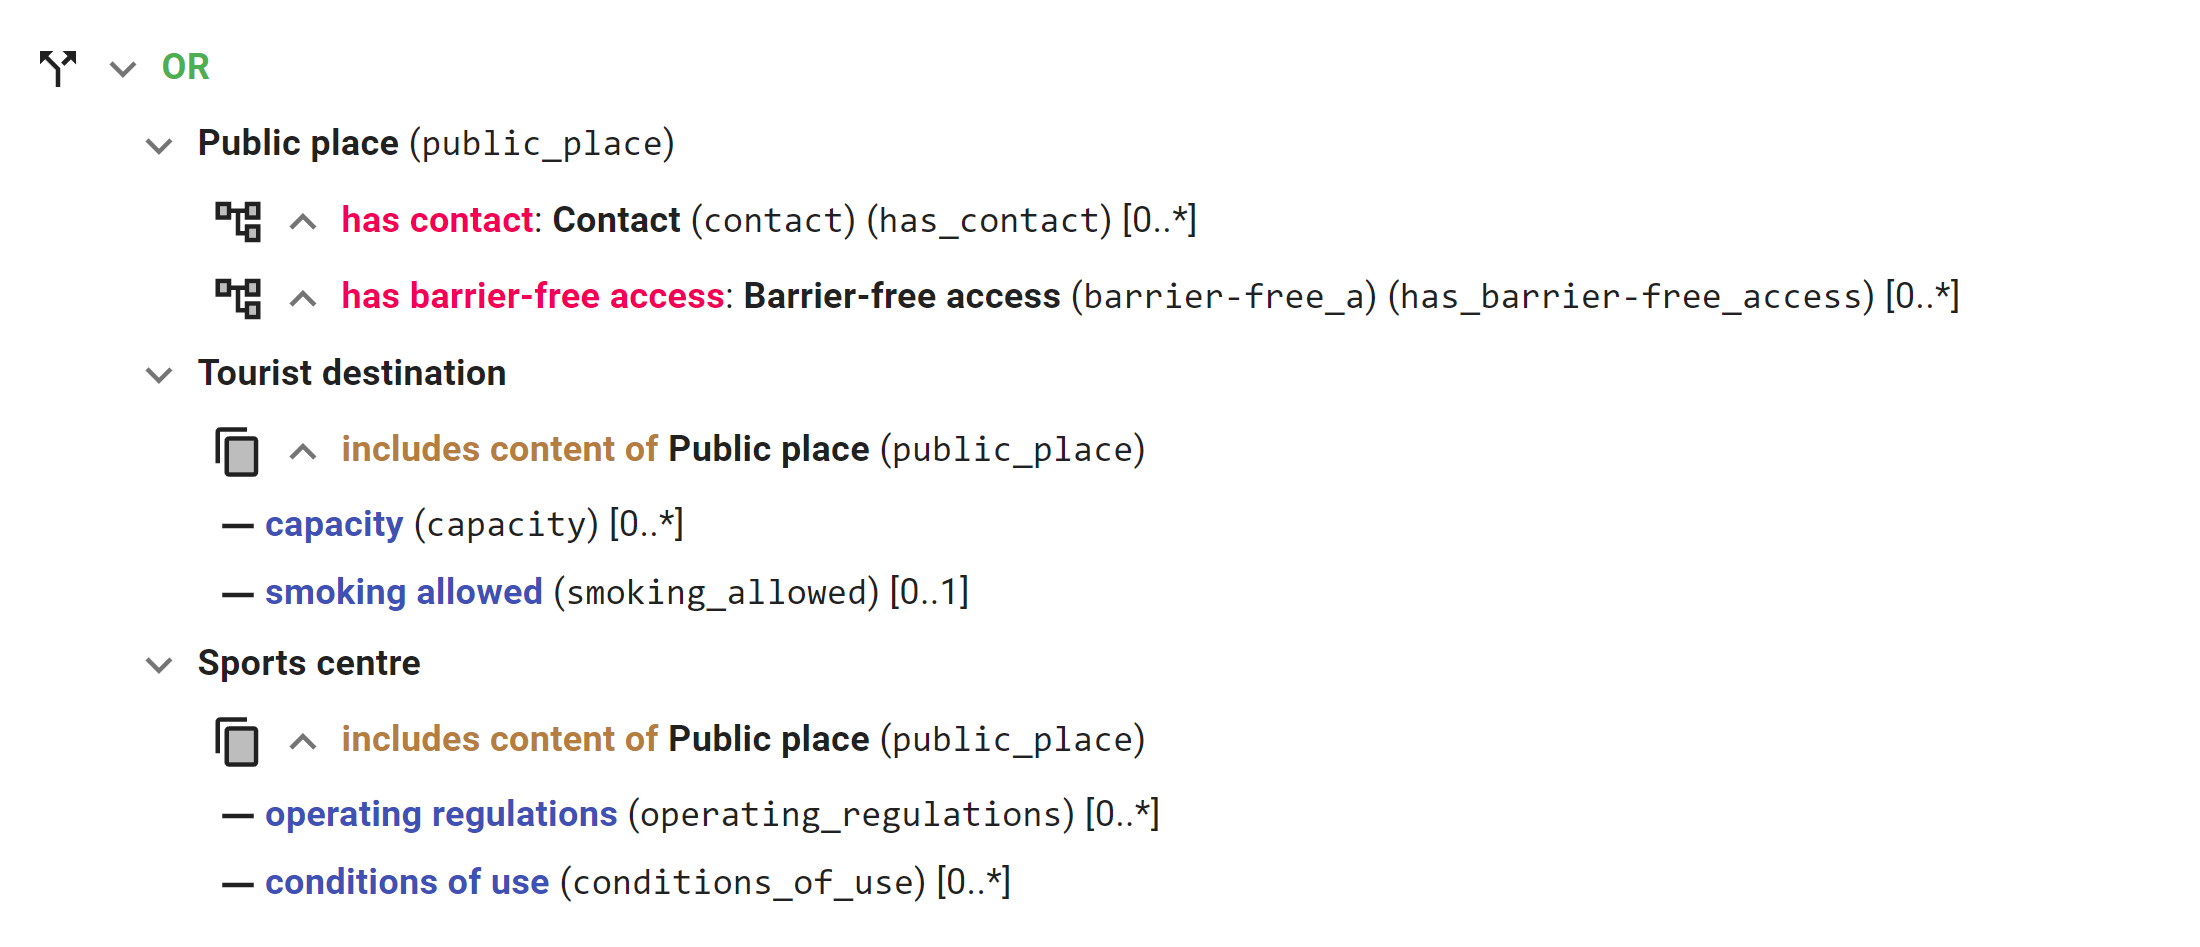
\includegraphics[width=\textwidth]{img/or_inheritance_off.png}
    \caption{General schema with OR in the root of the schema and several includes.}
  \end{subfigure}
  \begin{subfigure}[b]{\textwidth}
    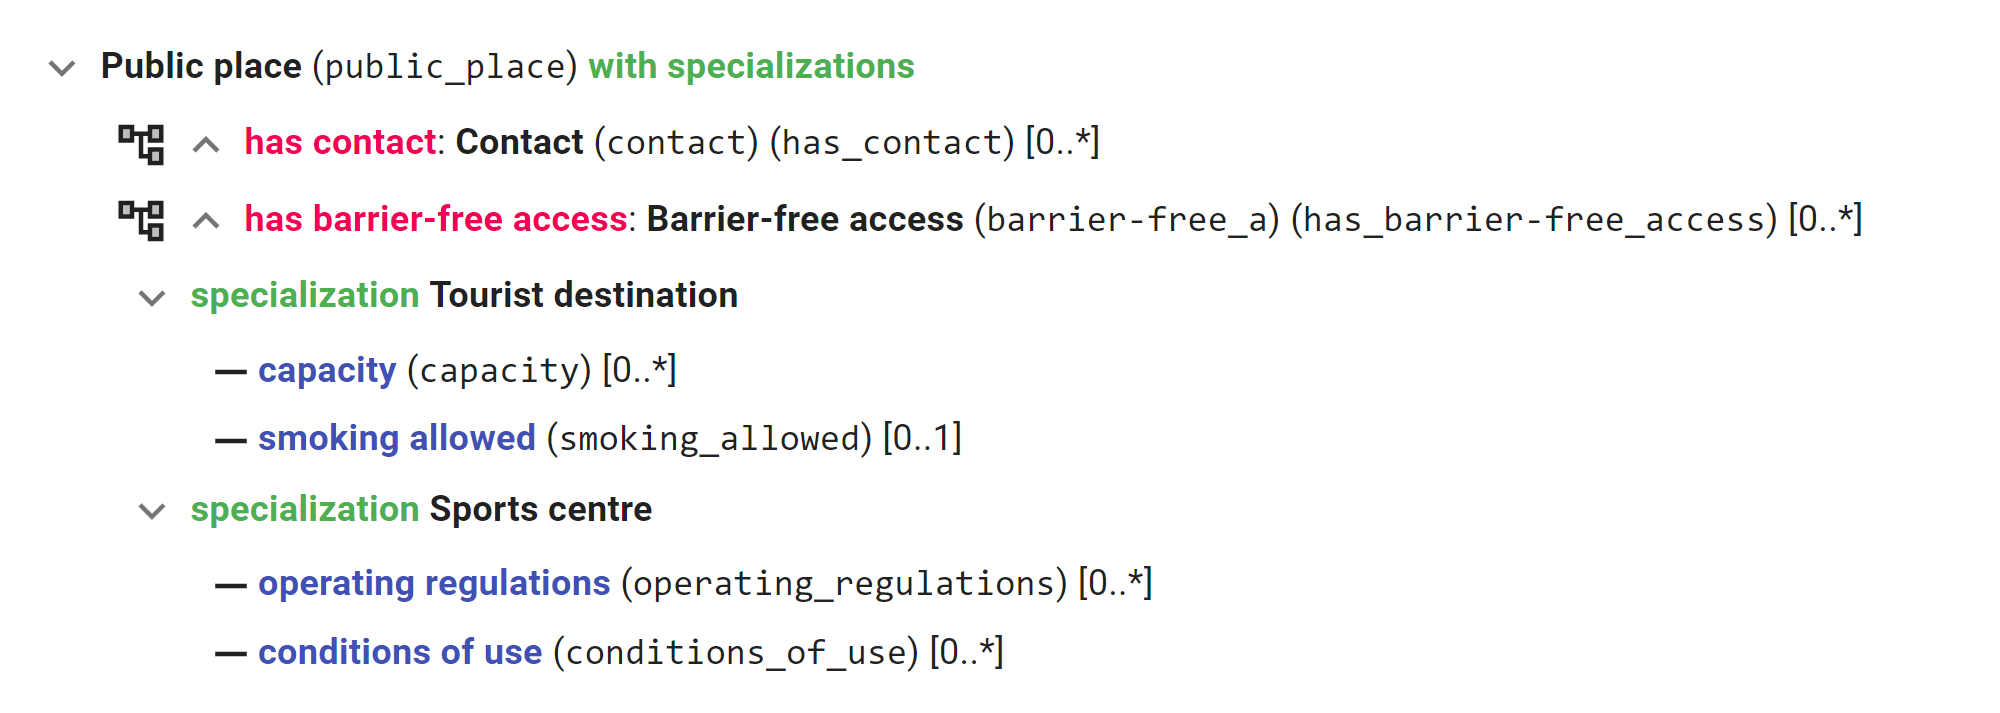
\includegraphics[width=\textwidth]{img/or_inheritance.png}
    \caption{Same general schema visualized as one base class with specializations.}
  \end{subfigure}
  \caption{Screenshots from the tool comparing a general schema of a Public place that has two specializations according to \autoref{requirement:inheritance}. The variants shows the raw view, consisting of OR and include, and the user-friendly view that hides those constructs. The example shows one of FOSes that we are trying to model. For the purpose of this example, the schema was simplified, some classes were contracted, and labels were translated to English.}
  \label{fig:screenshot-comparison}
\end{figure}
\vfill

\begin{figure}
  \centering
  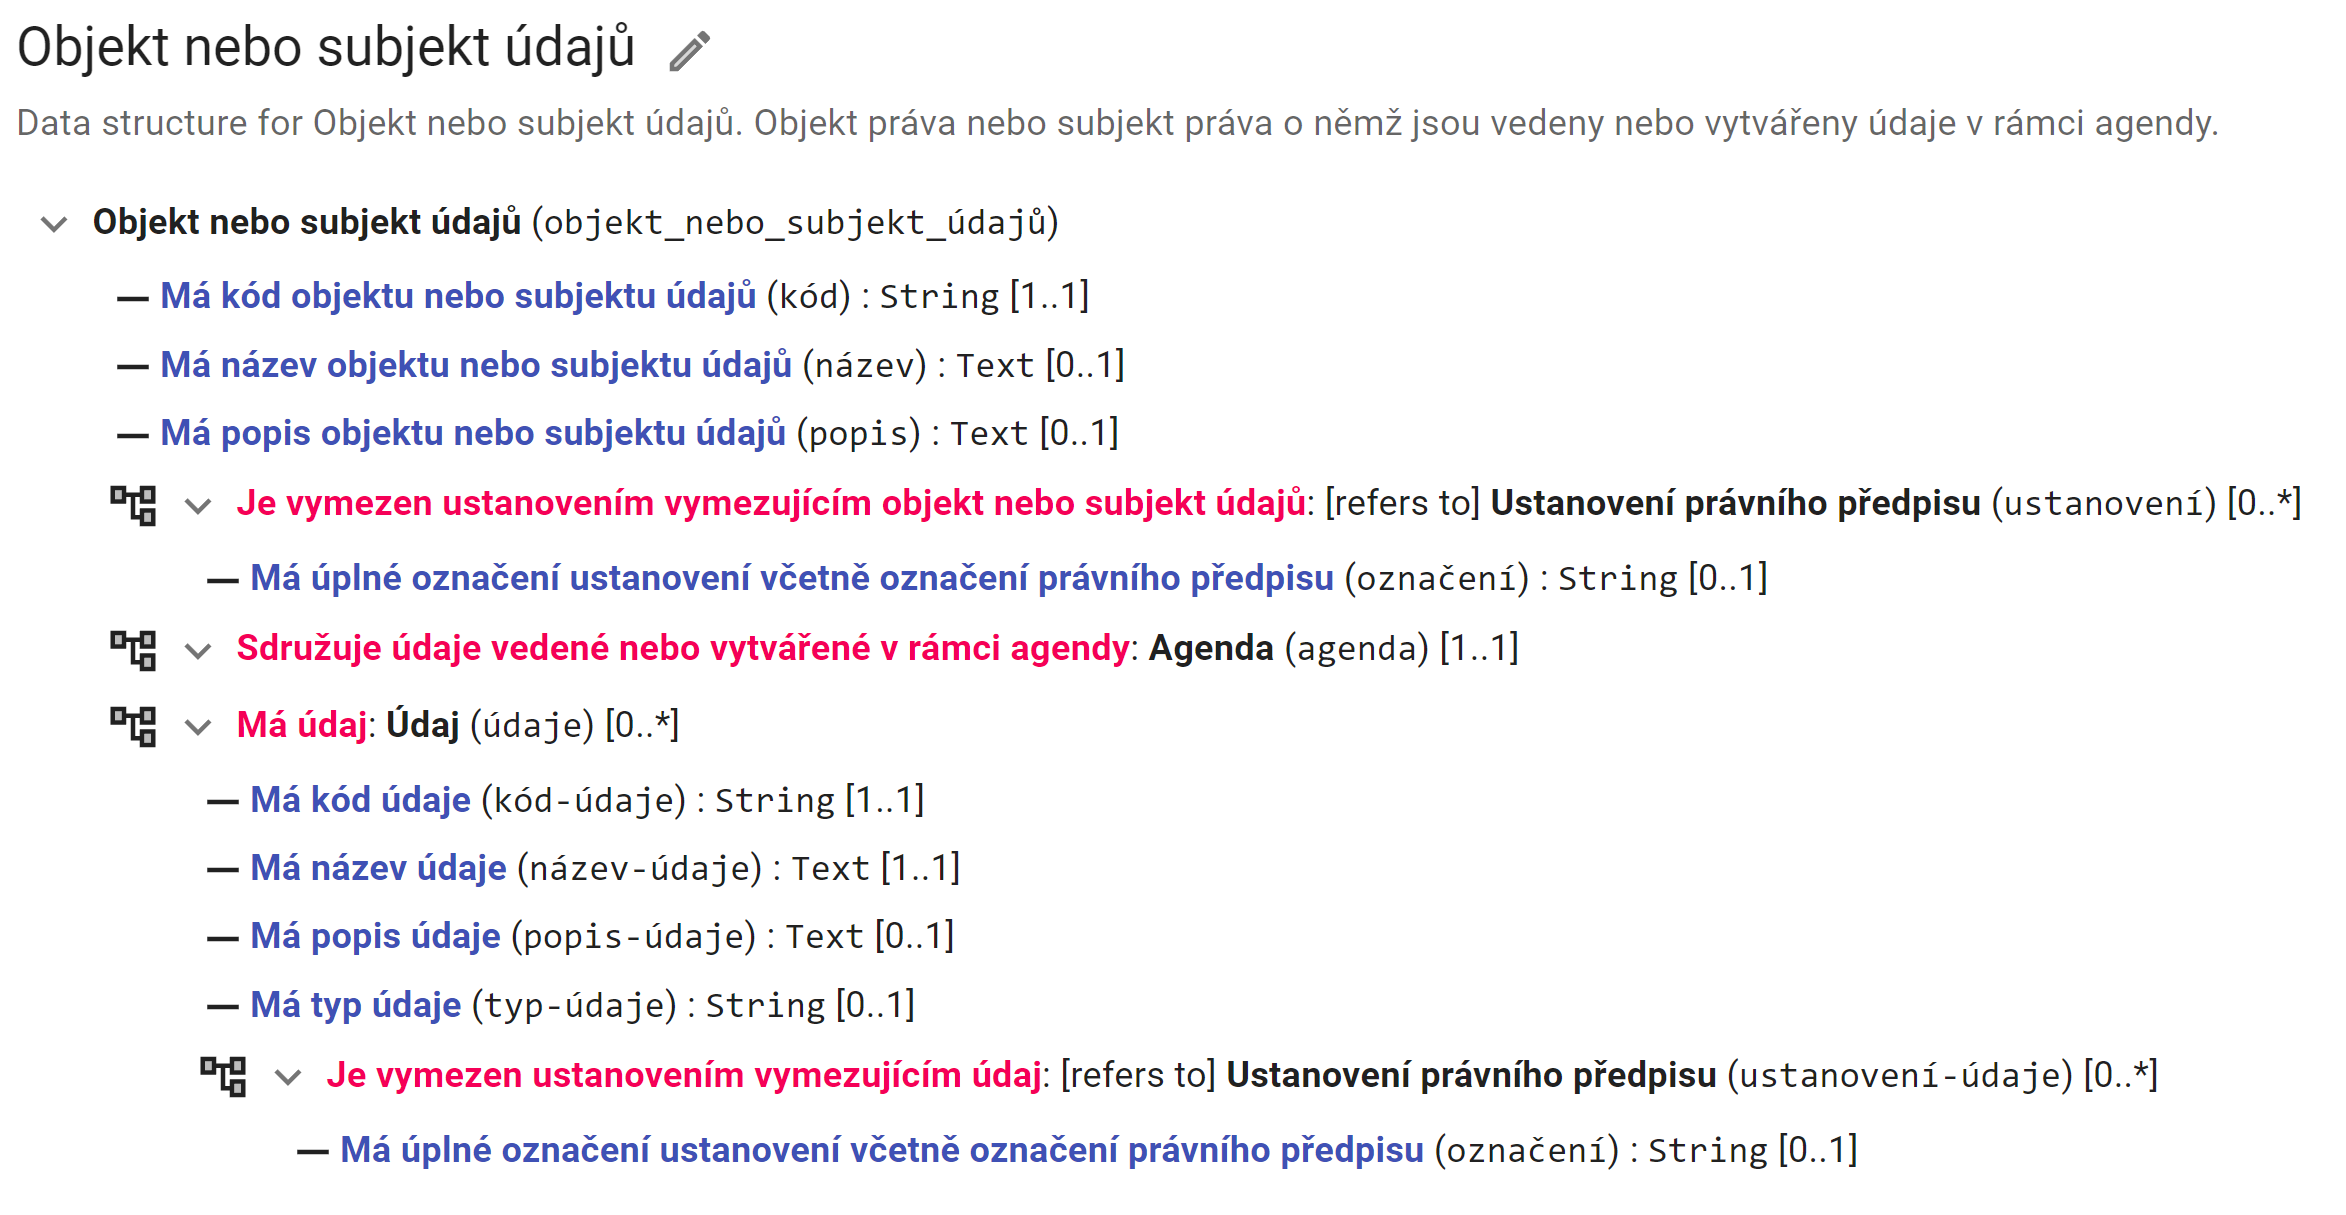
\includegraphics[width=\textwidth]{img/objekt_nebo_subjekt.png}
  \caption{Real example of a general schema of one of the RPP FOSes, that were described in \autoref{sec:register-of-rights-and-obligations}. You can see, that the schema consists of only few associations and attributes. There are two references to the ohter schema denoted by \textit{[refers to]} text.}
  \label{fig:screenshot}
\end{figure}
%
%\section{First Attachment}

\openright
\end{document}
